\documentclass[a4paper,11pt]{article}
\author{ 杨旭鹏  \  PB17000234}
\date{2019年秋季}
\title{计算物理A 第十二题}

\usepackage{ctex}
\usepackage{amsmath}
\usepackage{amsfonts}
\usepackage{graphicx}
\usepackage{epstopdf}
\usepackage{lastpage}
\usepackage{hyperref}
\usepackage{listings}
\RequirePackage{xcolor}
\usepackage{appendix}
\usepackage{caption2}
\usepackage{subfigure}
\usepackage{float}
\usepackage{verbatim}
\makeatletter\def\@captype{table}\makeatother

\definecolor{dkgreen}{rgb}{0,0.6,0}
\definecolor{gray}{rgb}{0.5,0.5,0.5}
\definecolor{mauve}{rgb}{0.58,0,0.82}

\lstset{
  frame=tb,
  aboveskip=3mm,
  belowskip=3mm,
  showstringspaces=false,
  columns=flexible,
  framerule=1pt,
  rulecolor=\color{gray!35},
  backgroundcolor=\color{gray!5},
  basicstyle={\small\ttfamily},
  numbers=left,
  numberstyle=\tiny\color{gray},
  keywordstyle=\color{blue},
  commentstyle=\color{dkgreen},
  stringstyle=\color{mauve},
  breaklines=true,
  breakatwhitespace=true,
  tabsize=3,            
  }



\begin{document}
\maketitle
\tableofcontents

\section{题目描述}
以$x_{n+1}=\lambda sin(\pi x_{n})$为迭代方程:

\begin{description}
\item[(1)] 画出系统状态随参数$\lambda$的变化图,要求包括定括定值状态、倍周期分叉和混沌状态;
\item[(2)]列出各个倍周期分叉处的$\lambda$值,求相应的 Feigenbaum 常数。
\end{description}


\section{算法}
对⼀定区间内间隔为某一值$step$的每⼀个$\lambda$,任意选定$x$的初始值$x_{0}$,利用给定的迭代公式计算并输出$N$迭代后的后$n$个$x$的值$x_{N-n},x_{N-n+1}, \cdots ,x_{N}$。然后利用输出的数据画出$x-\lambda$图像即可。

对于找计算Feigenbaum常数所需的分岔值,对不同$\lambda$取值输出的后$n$个迭代值进行种类计数,找到不同个数的不动点所对应的参数$\lambda$取值。然后不断缩小区间,加大精度来找到比较精确的分岔值$\lambda_{m}$。


\section{程序使用方法}
此程序设计为参数在程序代码中直接赋值形式,每次需在程序源码中进行参数调整,进而编译运行,以简化每次输入的过程(重复运行时不用在此输入)。可供调整的参数包括参数$\lambda$的最大最小值,其每一步的步长,迭代次数$N$,输出迭代结果个数$n$,调整完参数后,编译运行,程序会自动输出不同参数$\lambda$对应的后$n$个迭代结果至文件(在同一文件中,顺序按$\lambda$从小到大排列)。

\section{程序结果与讨论}

\subsection{方程参数对于迭代结果影响的可视化结果}
最开始对方程的特性不了解,故先设定$step = 0.5$,$\lambda \in [-100,100]$得到:

\begin{figure}[!htbp]        
\centering
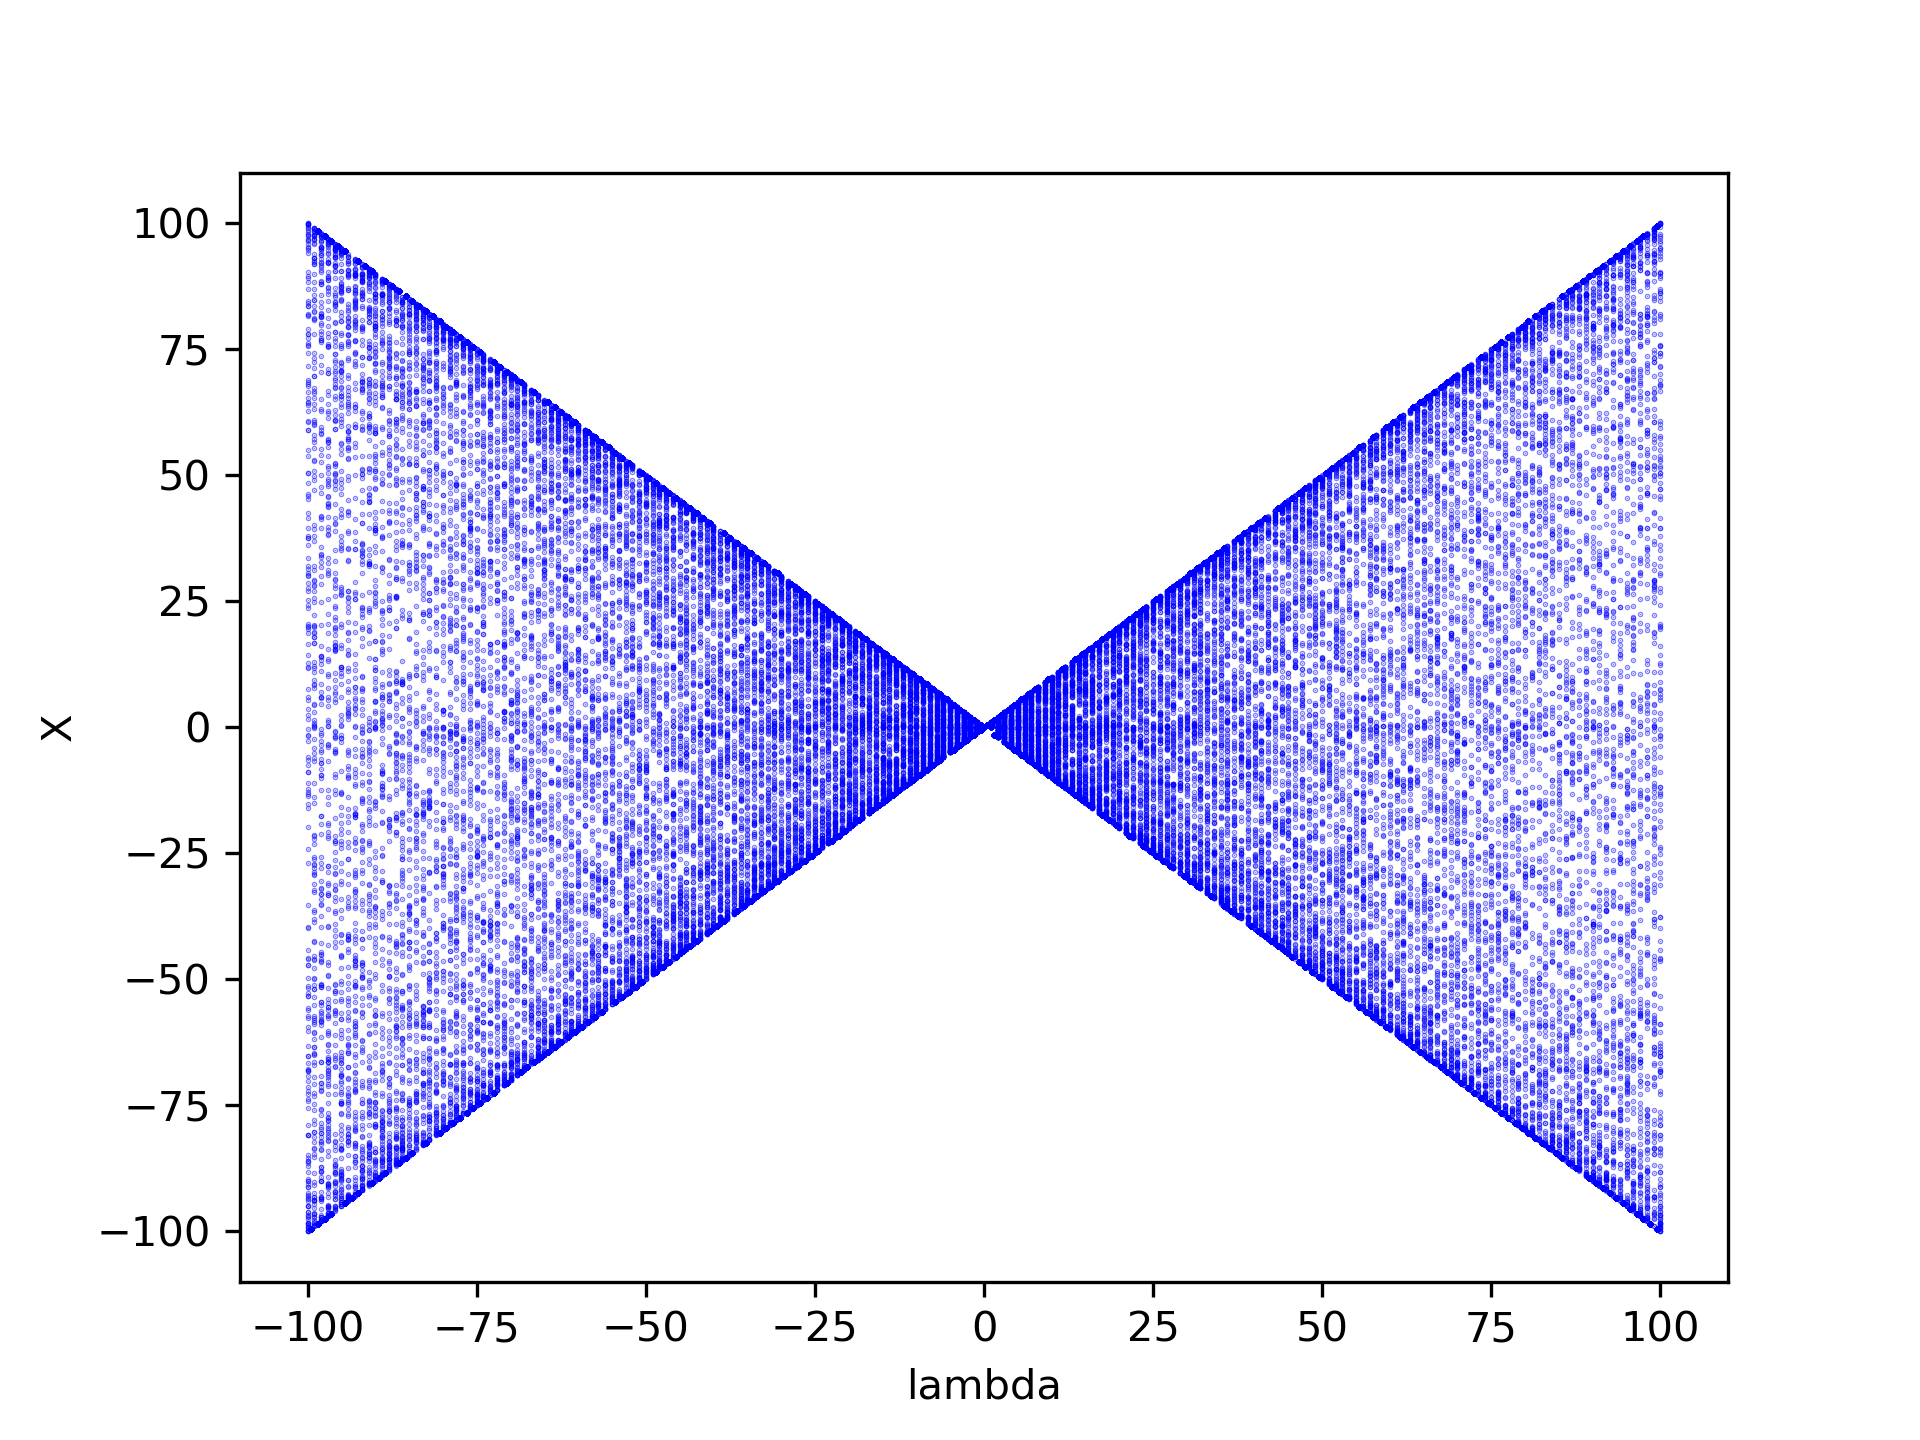
\includegraphics[bb= 0 0 450 370,width=9cm]{s=0.5.png}      
\caption{ $step = 0.5$,$\lambda \in [-100,100]$}      
\end{figure}

\newpage 发现此迭代方程只有在$0$附近收敛,在趋向负无穷和正无穷的过程中逐渐趋于混沌。

我们减小$\lambda$的范围至$[-10,10]$,并调小$step$至$0.01$得到:
\begin{figure}[!htbp]        
\centering
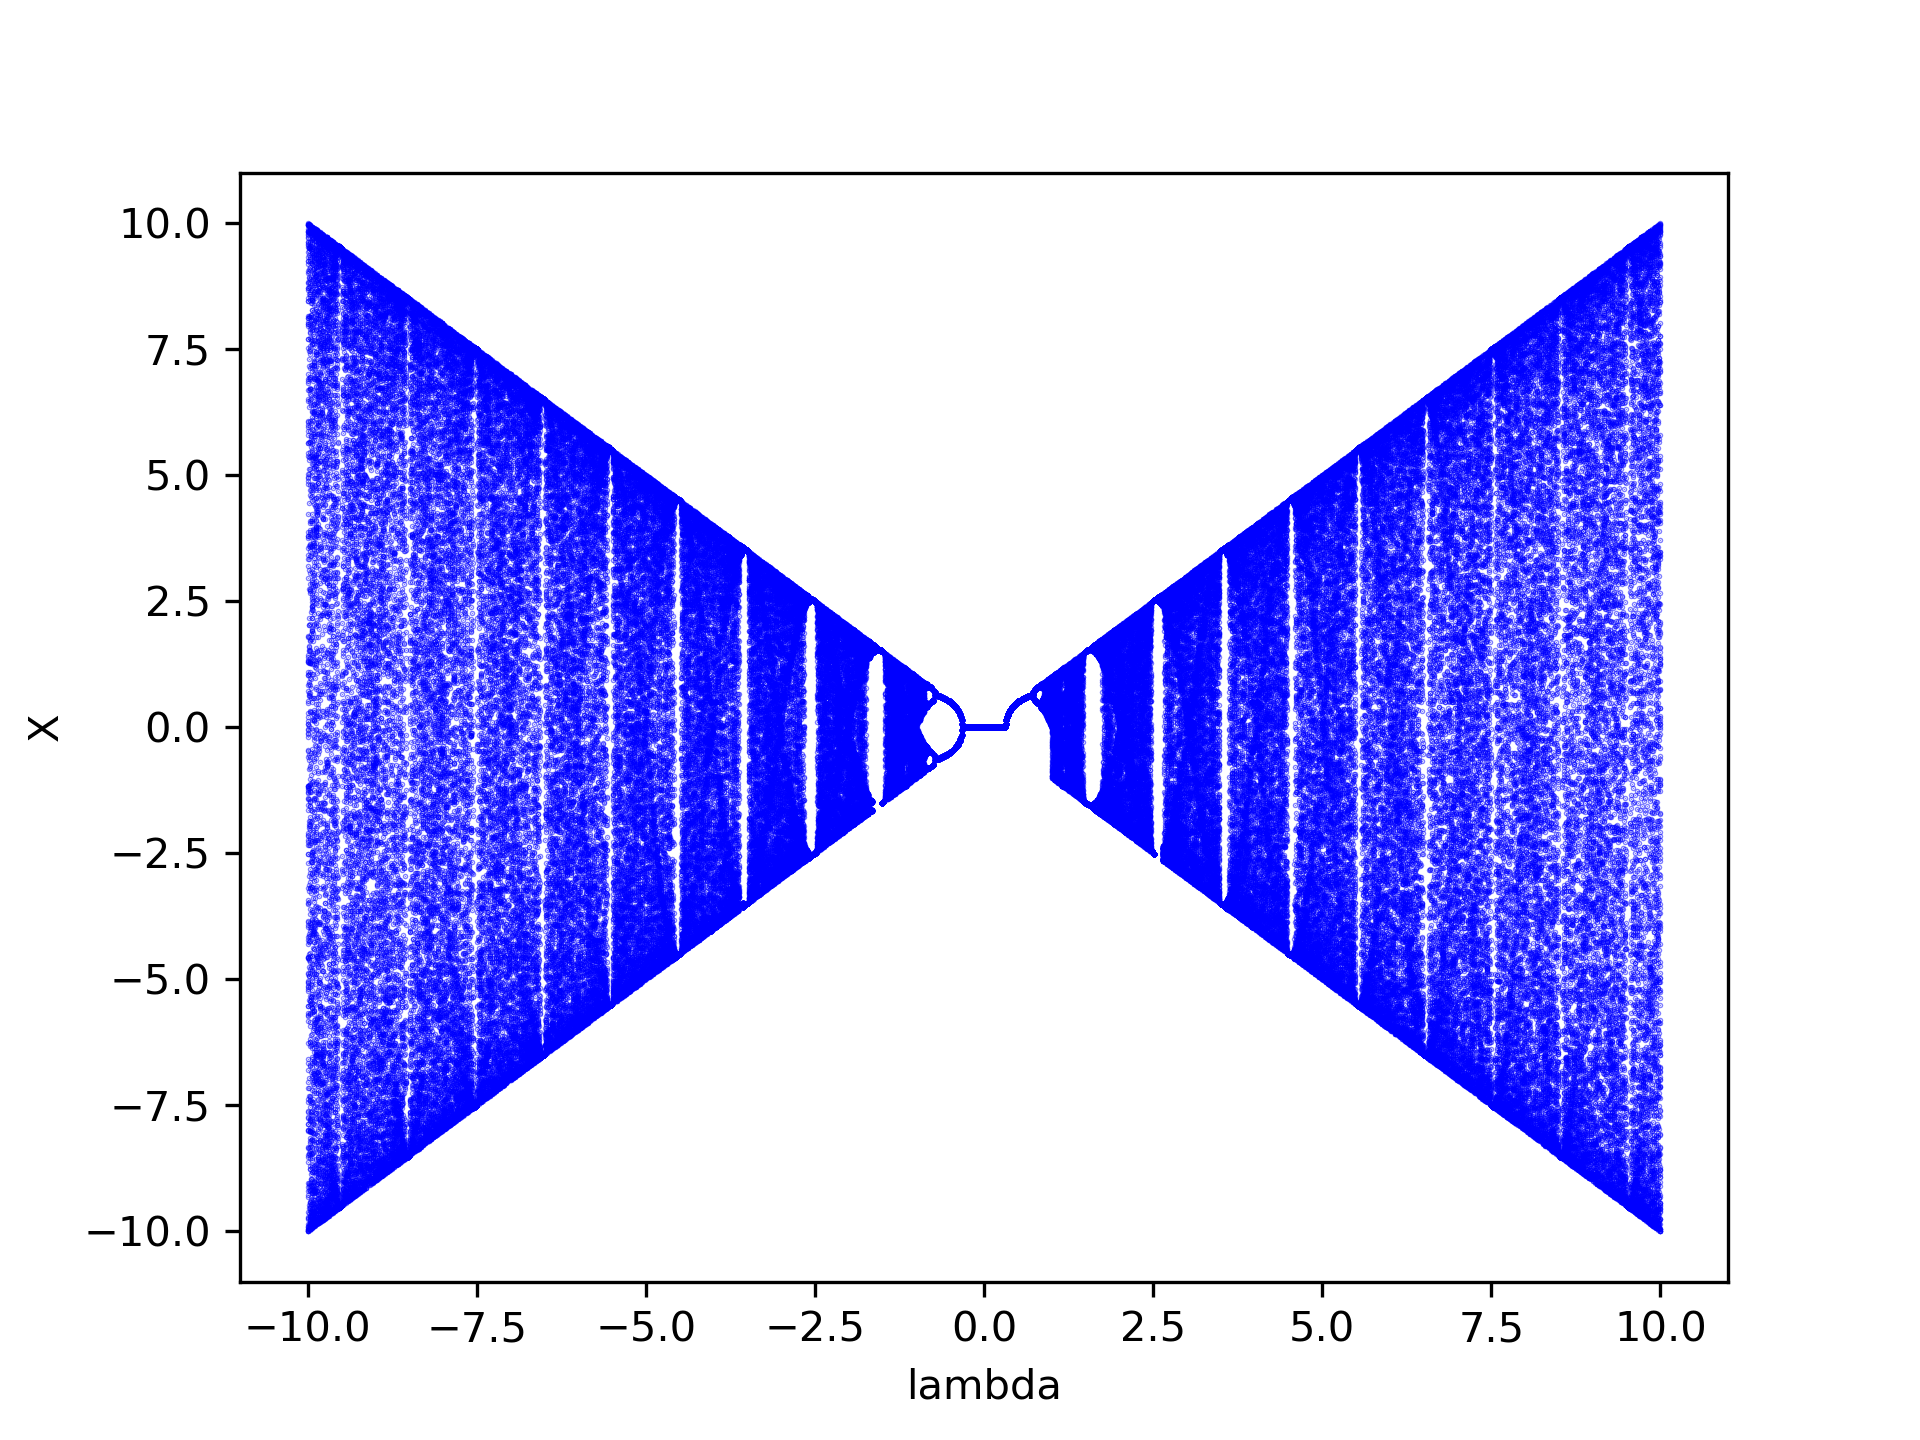
\includegraphics[bb= 0 0 450 370,width=9cm]{s=0.01.png}      
\caption{ $step = 0.01$,$\lambda \in [-10,10]$}      
\end{figure}

我们减小$\lambda$的范围至$[-1,1]$,并调小$step$至$0.001$得到:

\begin{figure}[!htbp]        
\centering
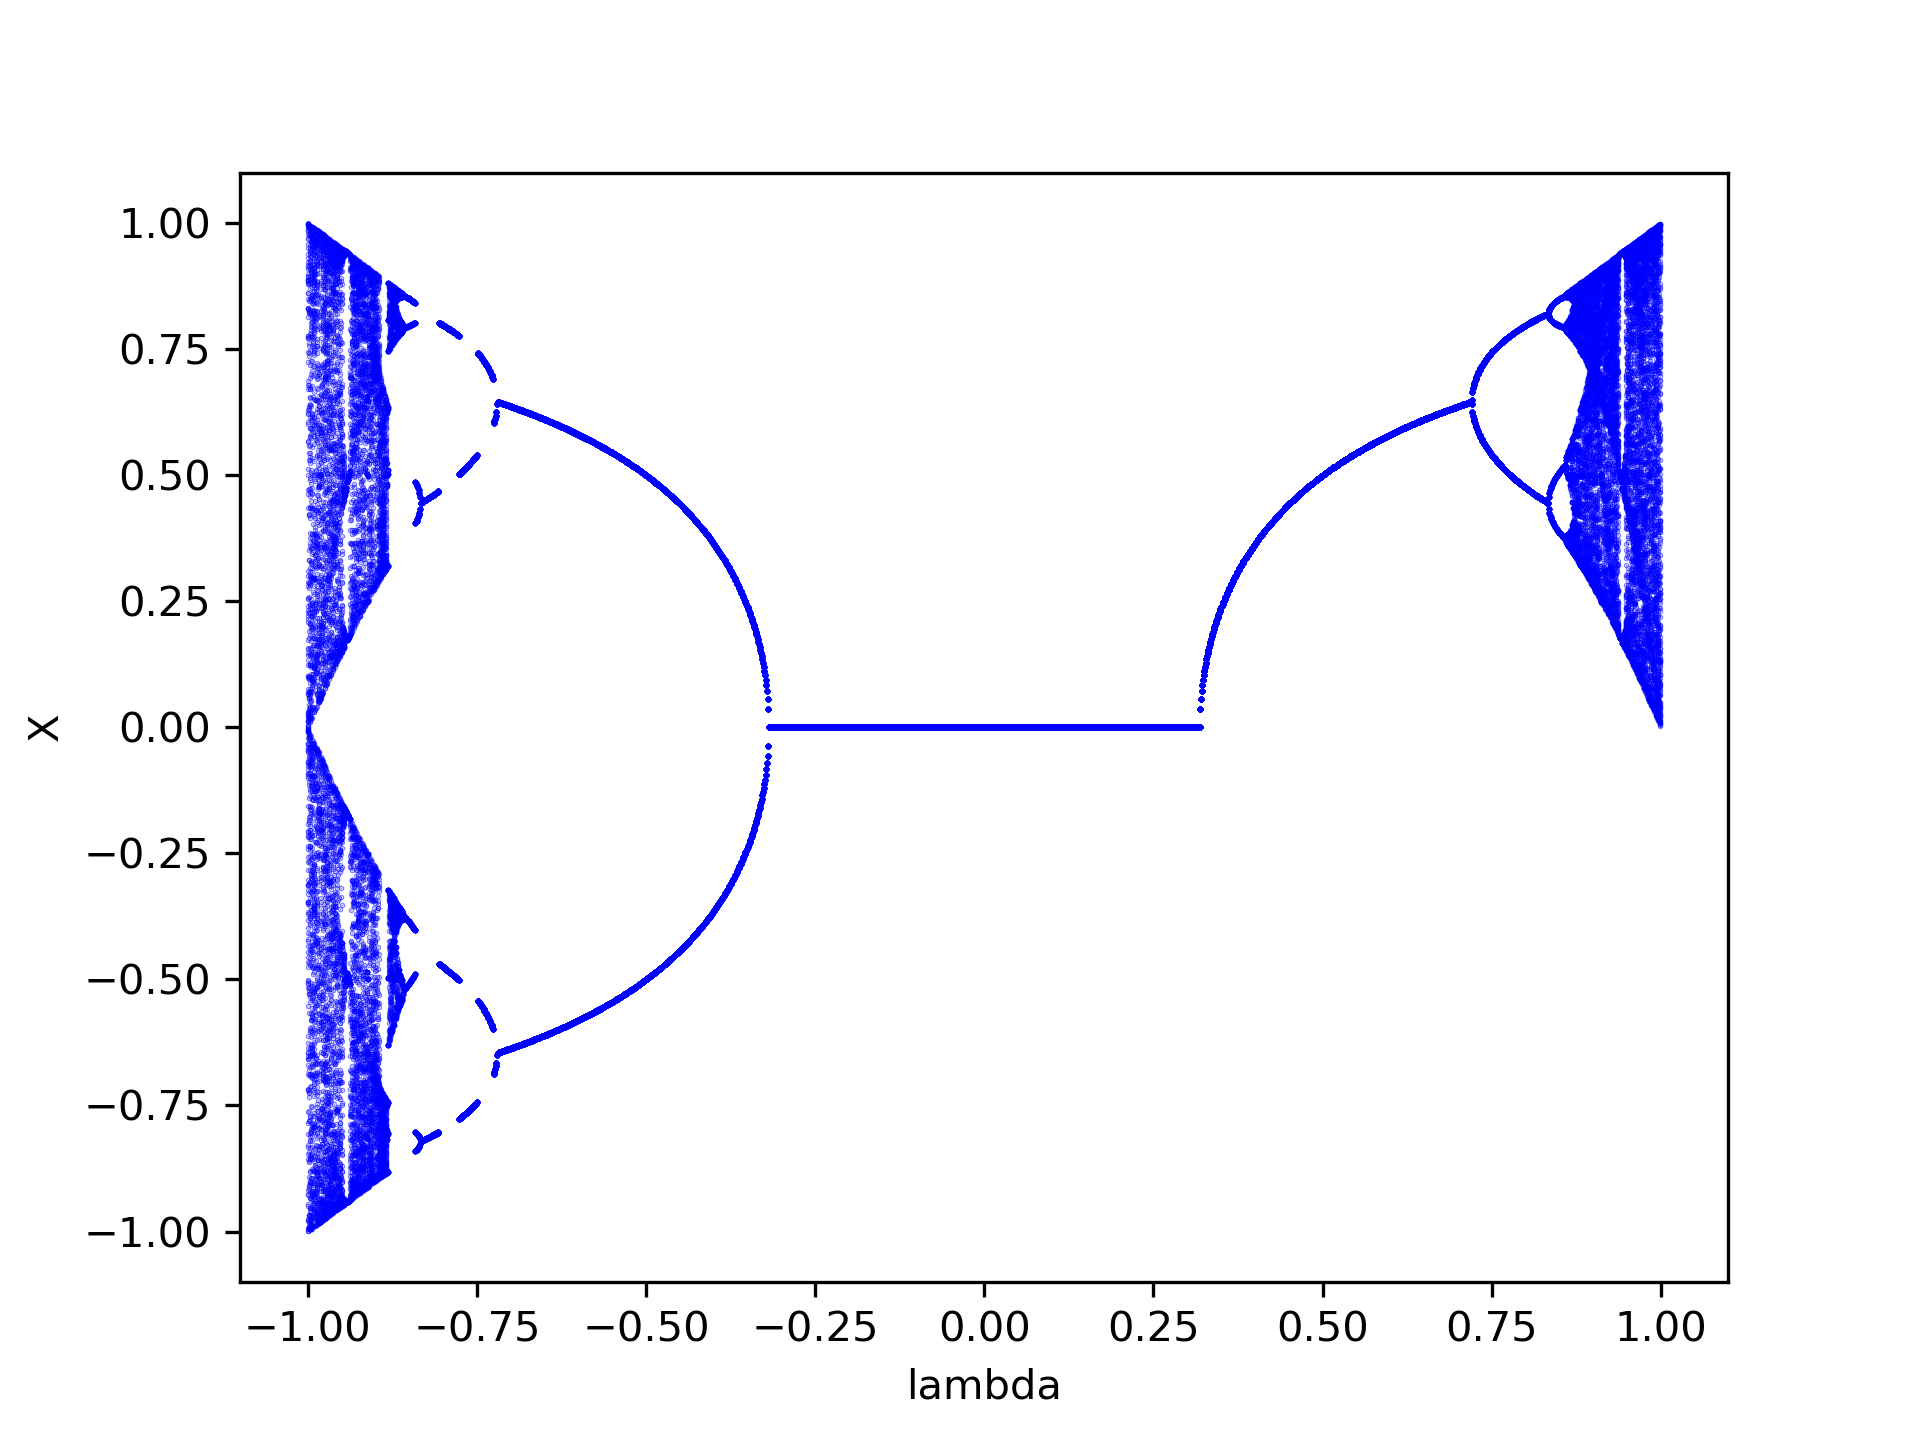
\includegraphics[bb= 0 0 450 370,width=9cm]{s=0.001.png}      
\caption{ $step = 0.001$,$\lambda \in [-1,1]$}      
\end{figure}

可以看到在0附近,迭代方程是收敛到0的,即所谓的“绝灭”。随着参数$\lambda$从0开始向无穷方向移动,方程从“绝灭”到一个不动点(定态)到2个不动点到4个不动点以此类推。我们将参数$\lambda$的范围一分为2来看有:



\begin{figure}[!htbp]        
\centering
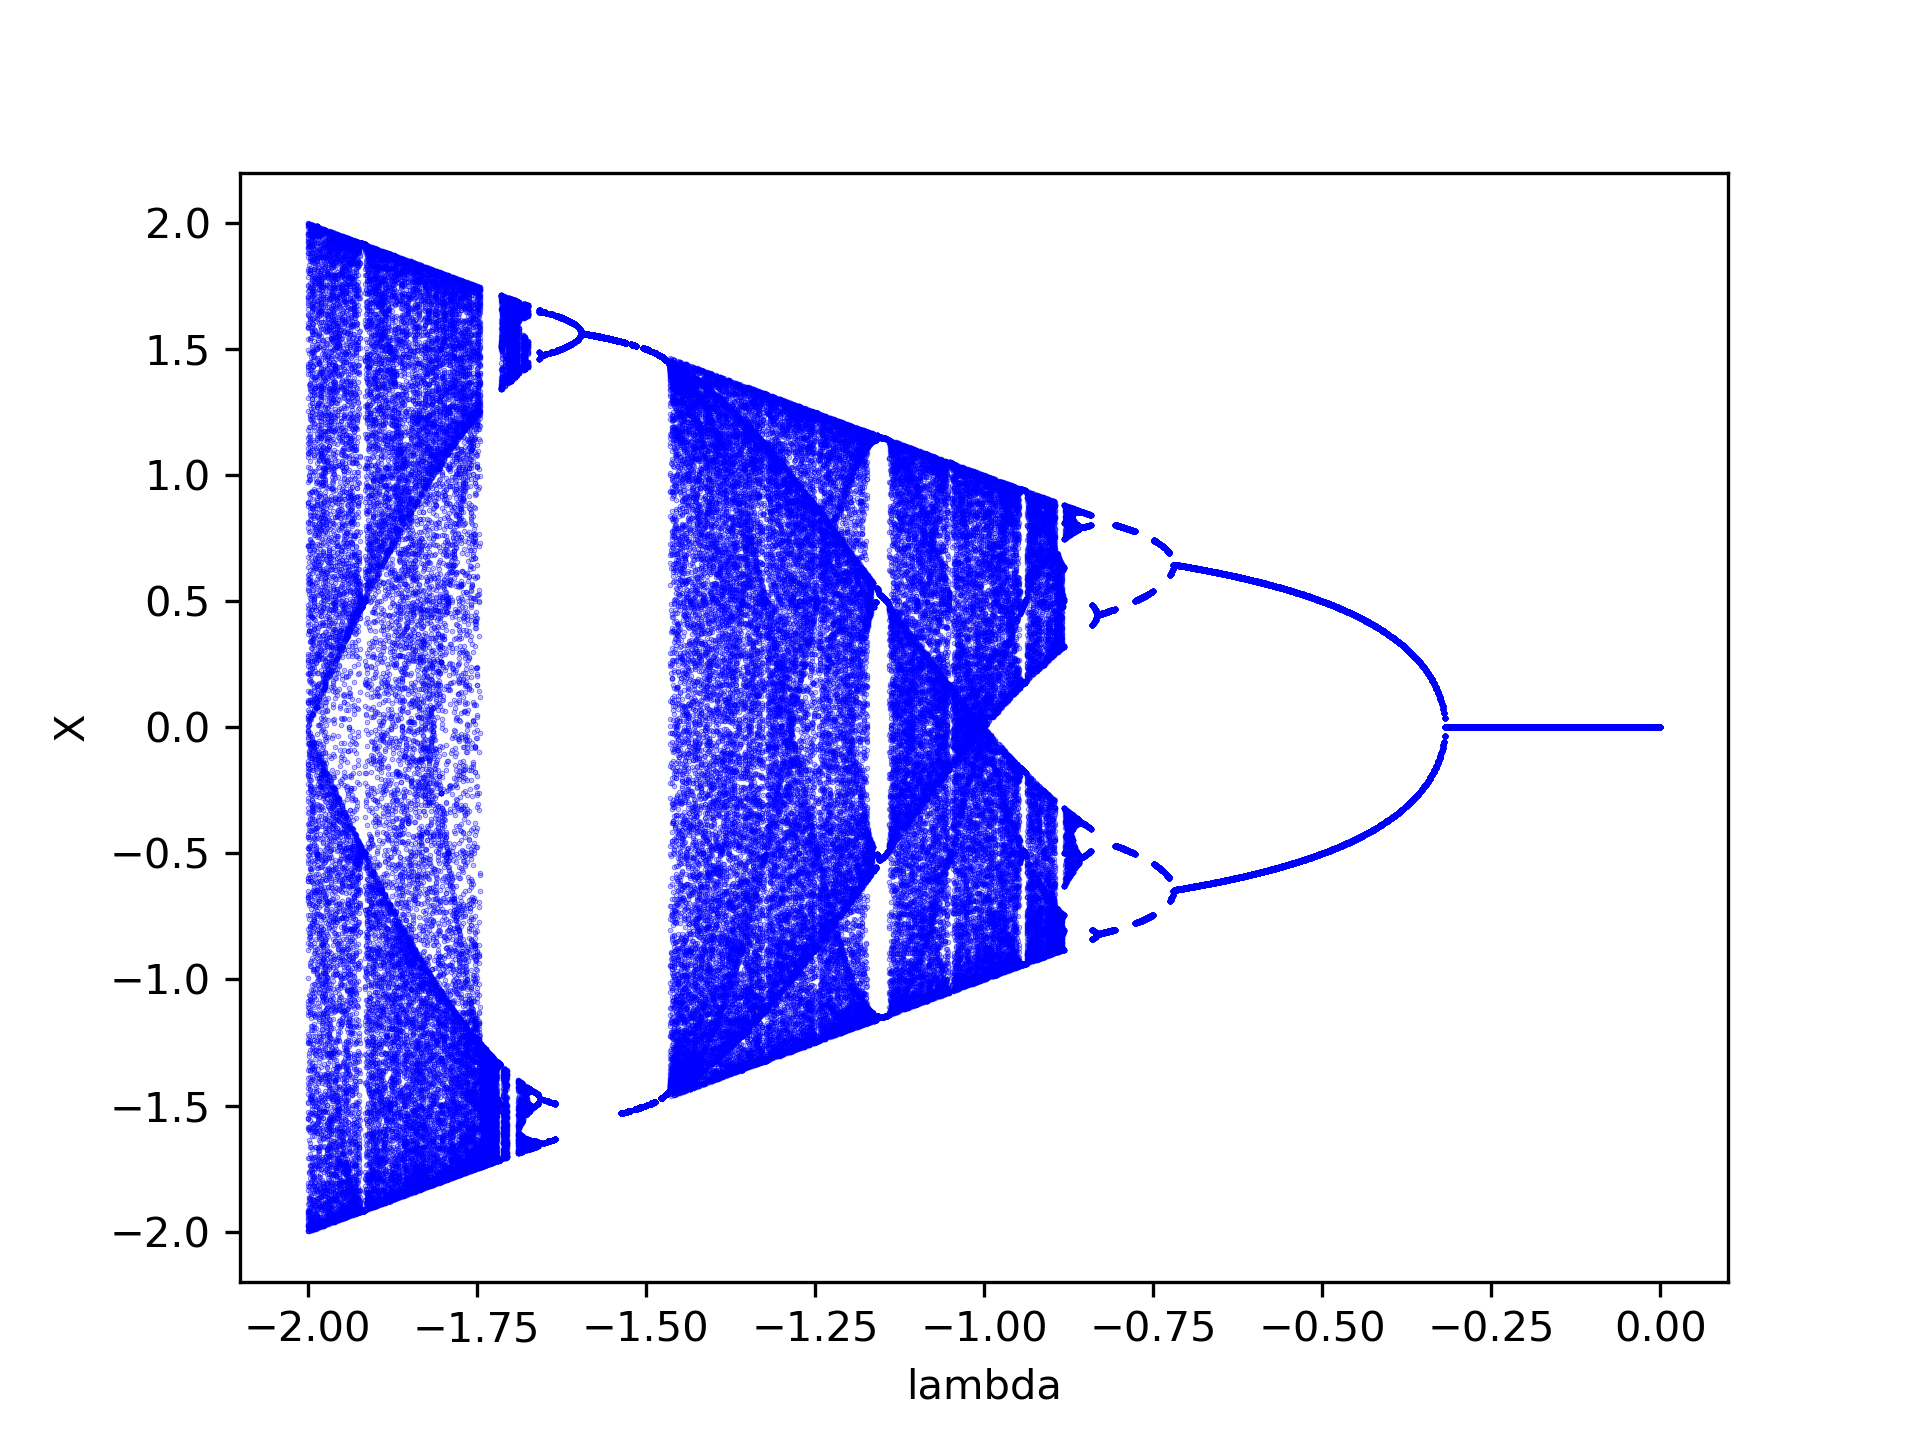
\includegraphics[bb= 0 0 450 370,width=9cm]{s=0.001-2.png}      
\caption{ $step = 0.001$,$\lambda \in [-2,0]$}      
\end{figure}

\newpage 可以看到在靠近0处,系统处于绝灭态,随着$\lambda$逐渐变小系统依次变成2分岔,4分岔,直到变为混沌态,之后又有周期窗口等现象。

\begin{figure}[!htbp]        
\centering
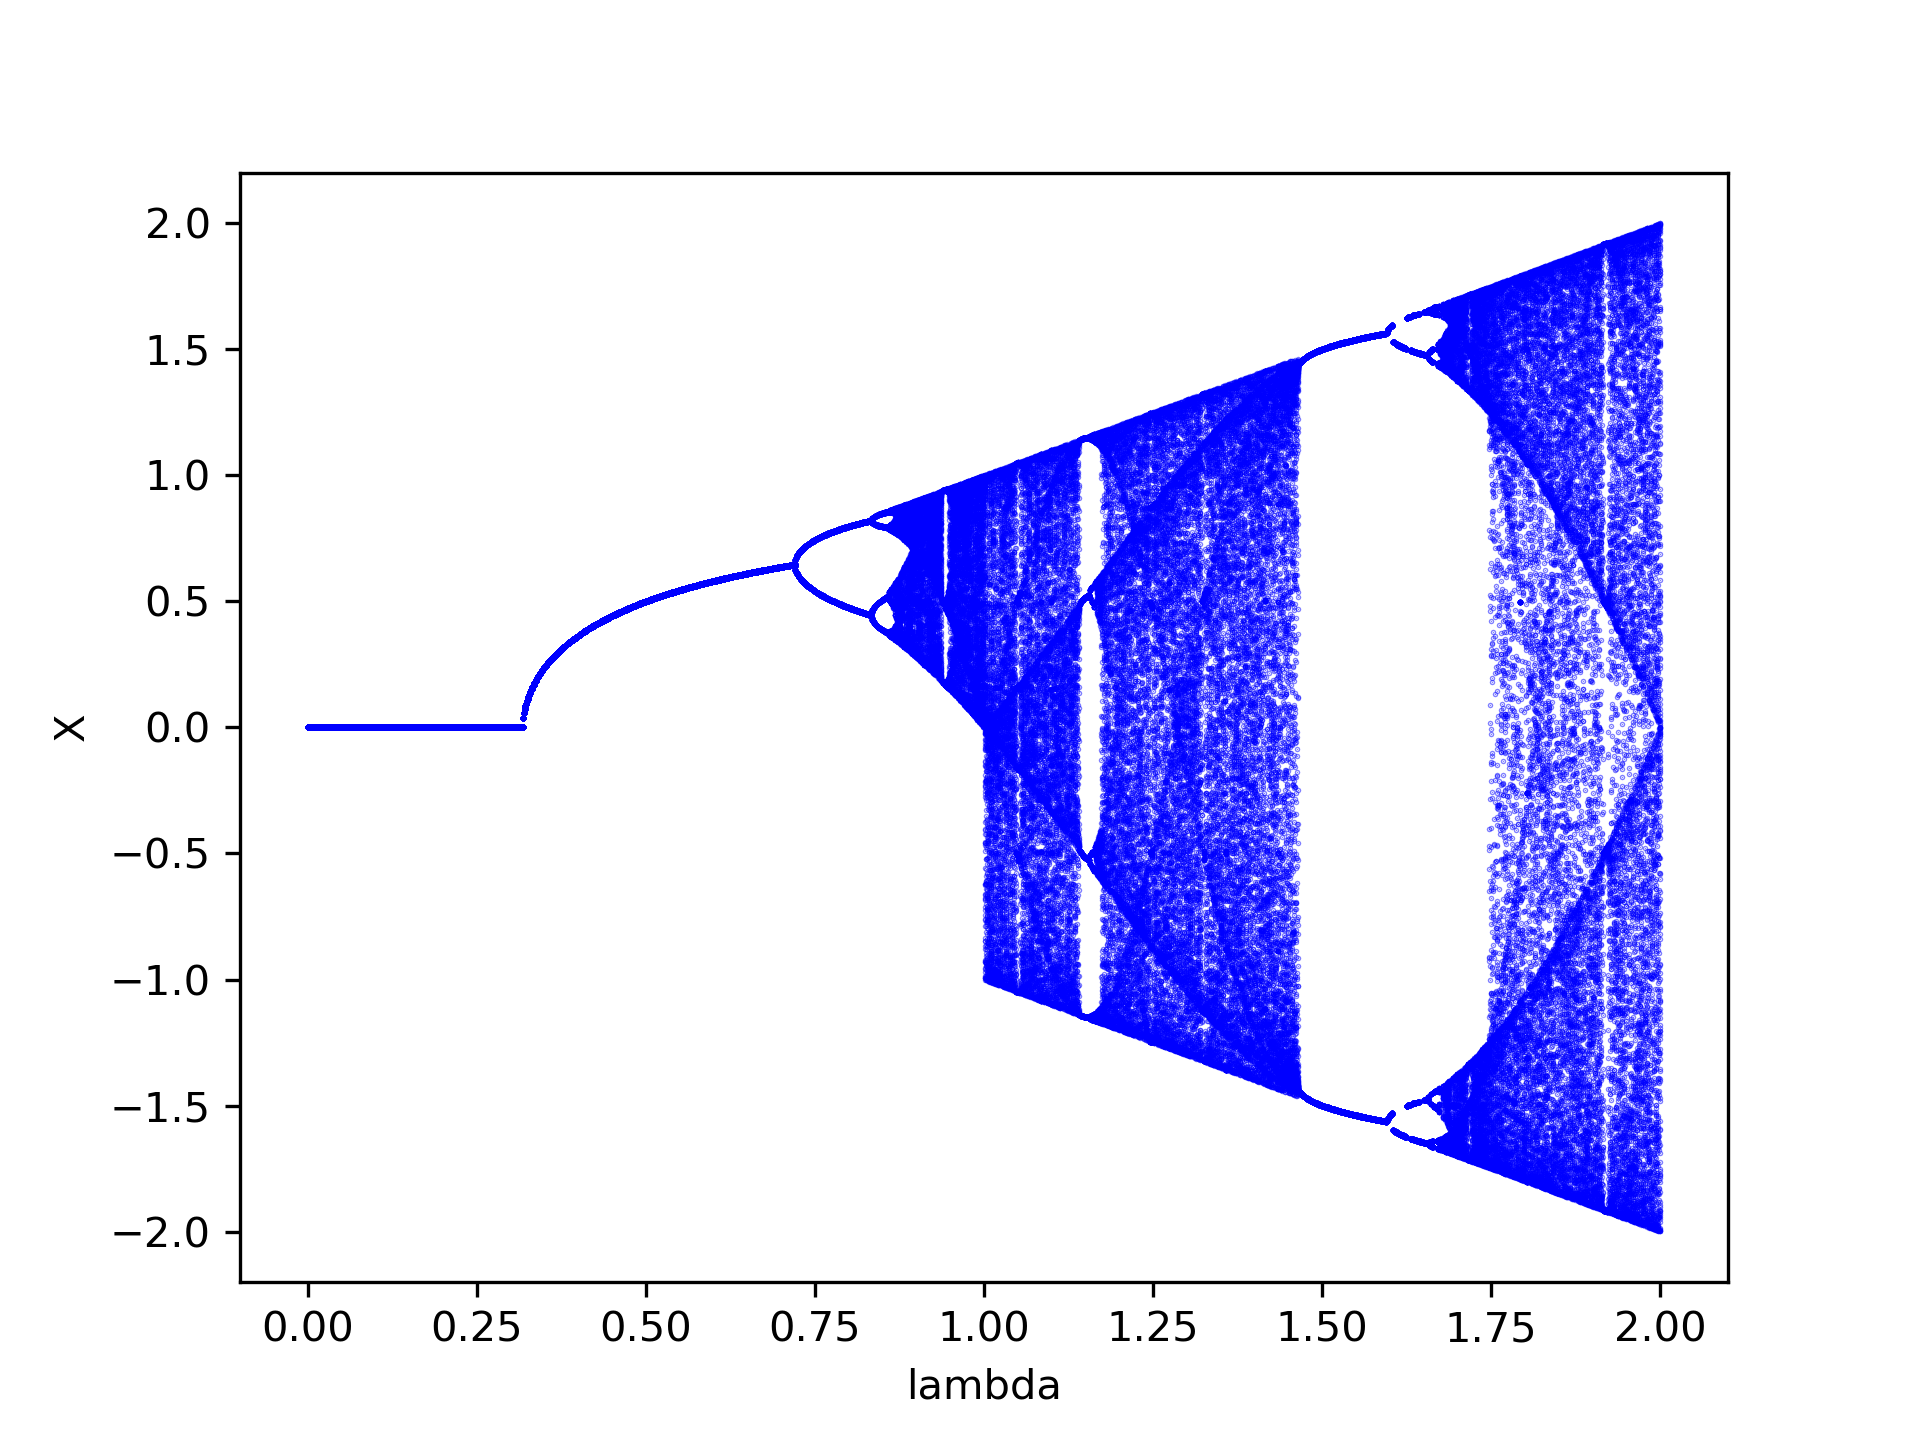
\includegraphics[bb= 0 0 450 370,width=9cm]{s=0.001-3.png}      
\caption{ $step = 0.001$,$\lambda \in [0,2]$}      
\end{figure}

\newpage 可以看到在靠近0处,系统处于绝灭态,随着$\lambda$逐渐变大系统依次变成定值态,2分岔,4分岔,直到变为混沌态,之后又有周期窗口等现象。

若将图形的一部分放大,我们期待能有分形的结构。下面展示对$\lambda < 0$的情况下部分图像的放大:


\begin{figure}[!htbp]        
\centering
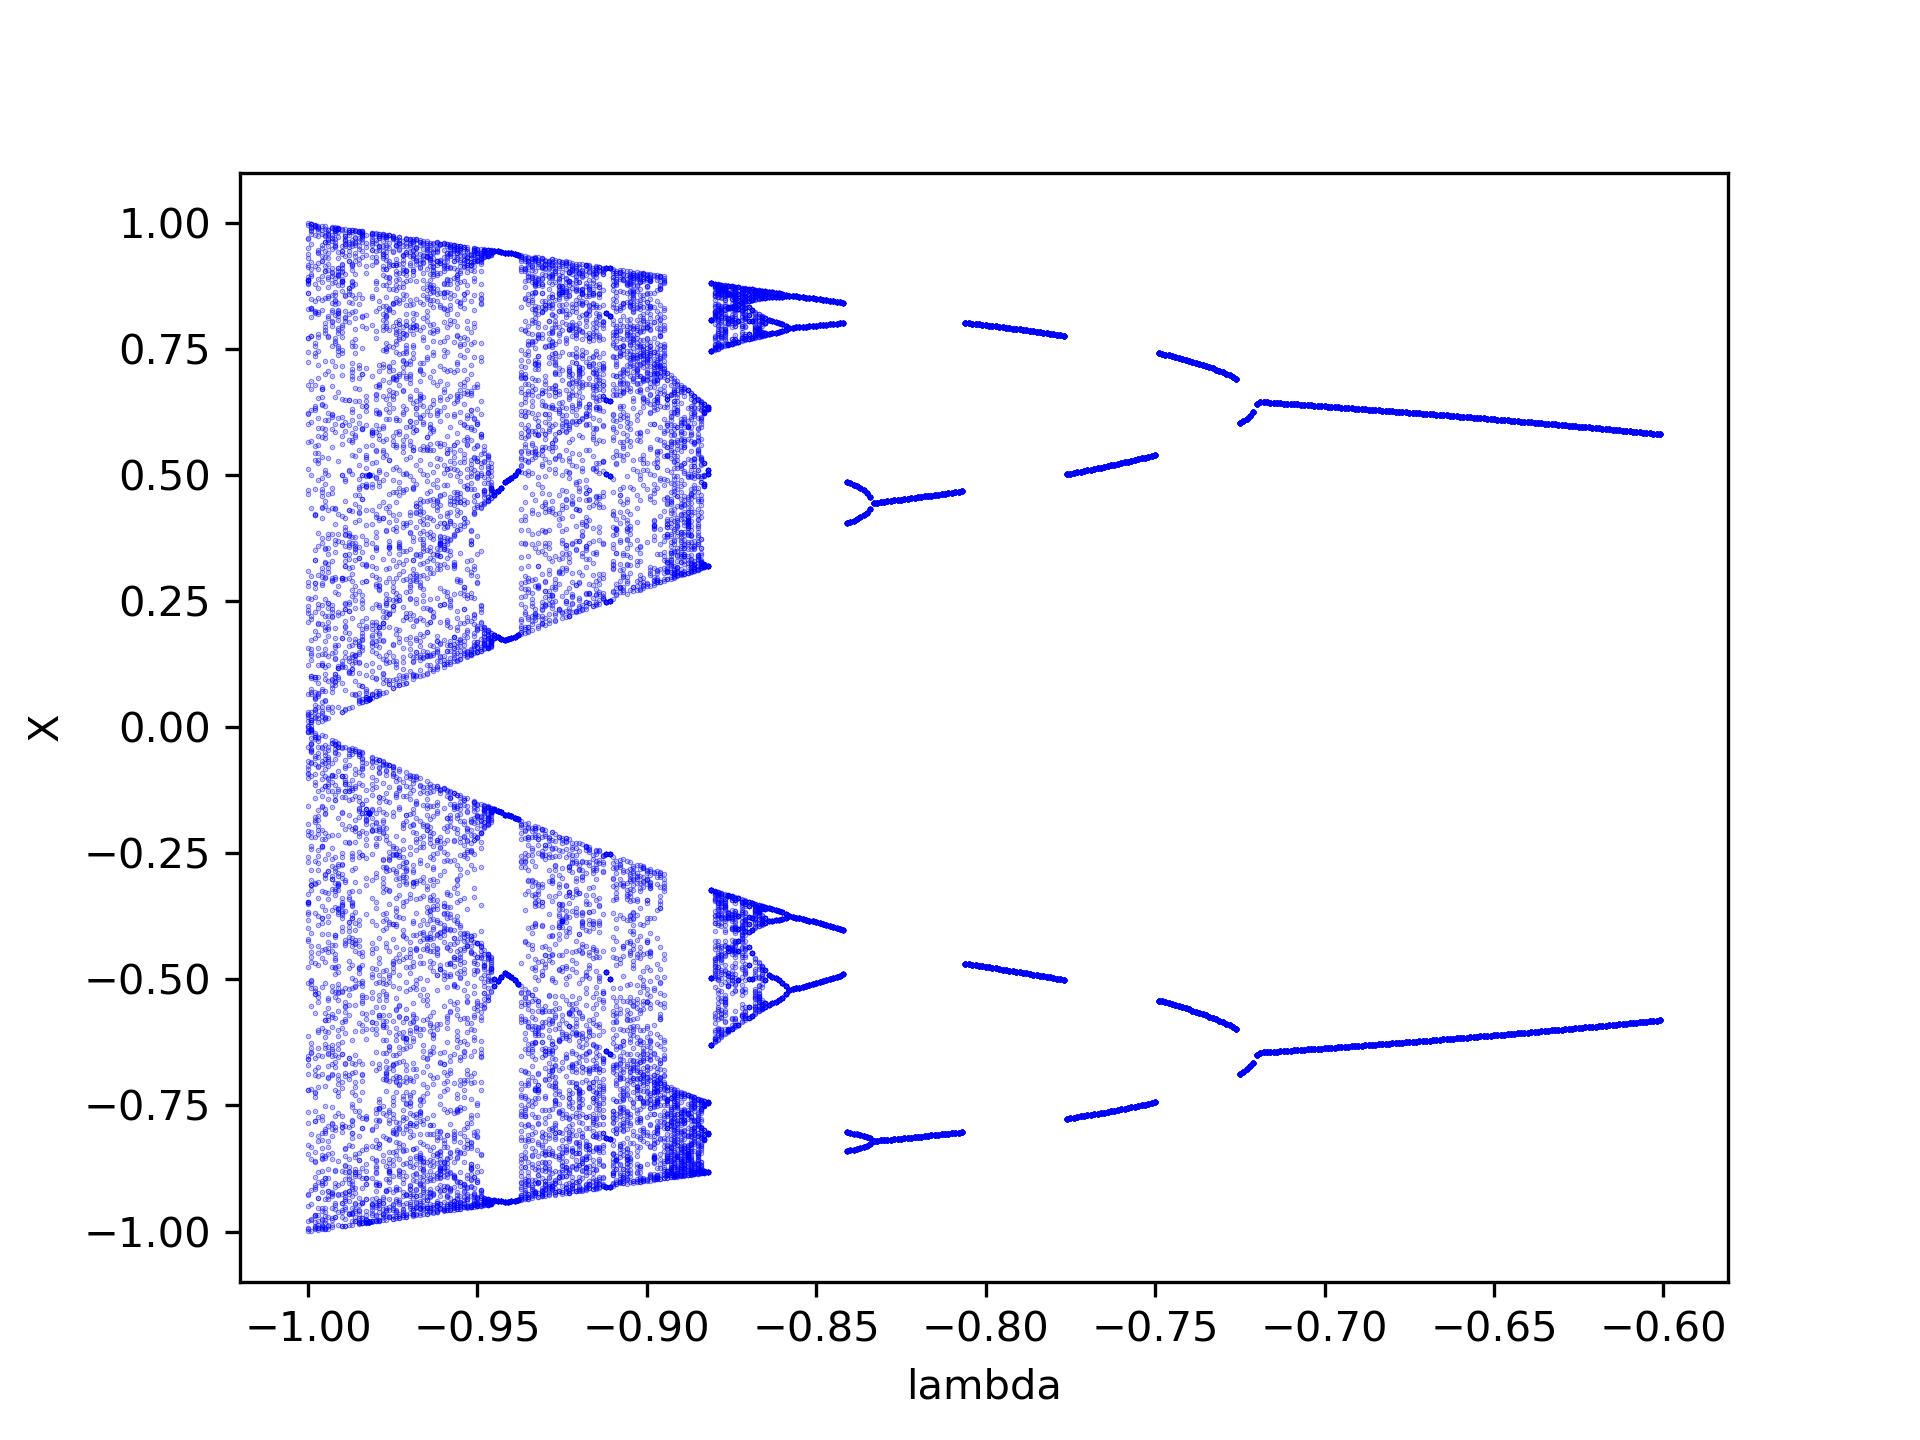
\includegraphics[bb= 0 0 450 370,width=9cm]{s=0.001-2-2.png}      
\caption{ $step = 0.001$,$\lambda \in [-1,-0.6]$}      
\end{figure}


\begin{figure}[!htbp]        
\centering
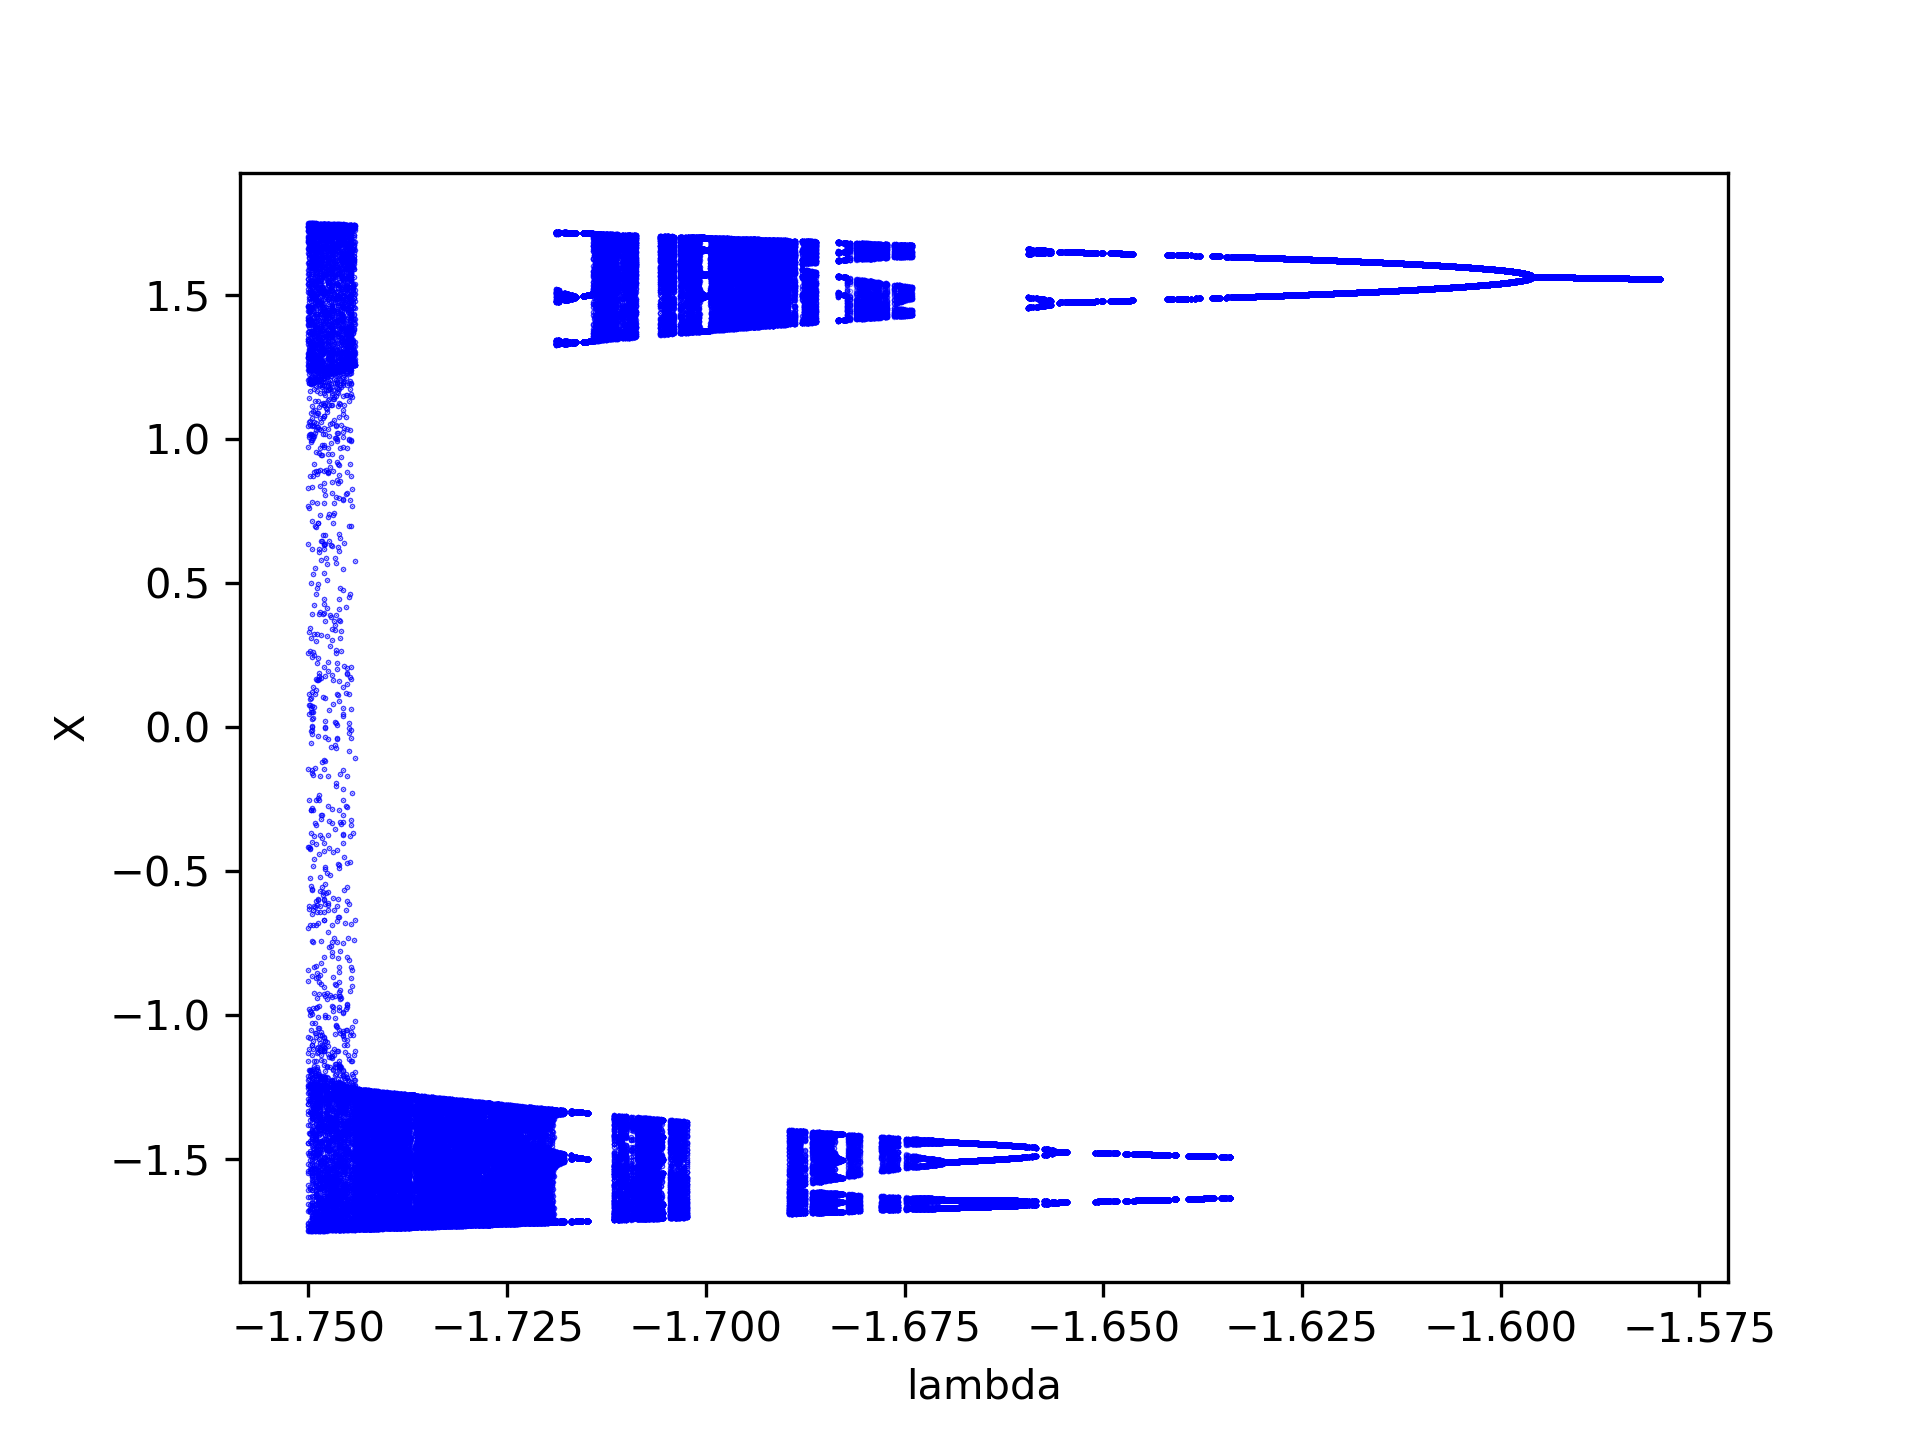
\includegraphics[bb= 0 0 450 370,width=9cm]{s=0.00001.png}      
\caption{ $step = 0.0001$,$\lambda \in [-1.75,-1.58]$}      
\end{figure}

\newpage
可以大致看出此图形的确有分形的结构。

我们还将$\lambda$在$[-2,0]$,$[0,2]$两个区间内以间隔为$0.001$做出迭代输出的后100个结果中的不同结果个数与参数$\lambda$的关系曲线:

\begin{figure}[!htbp]        
\centering
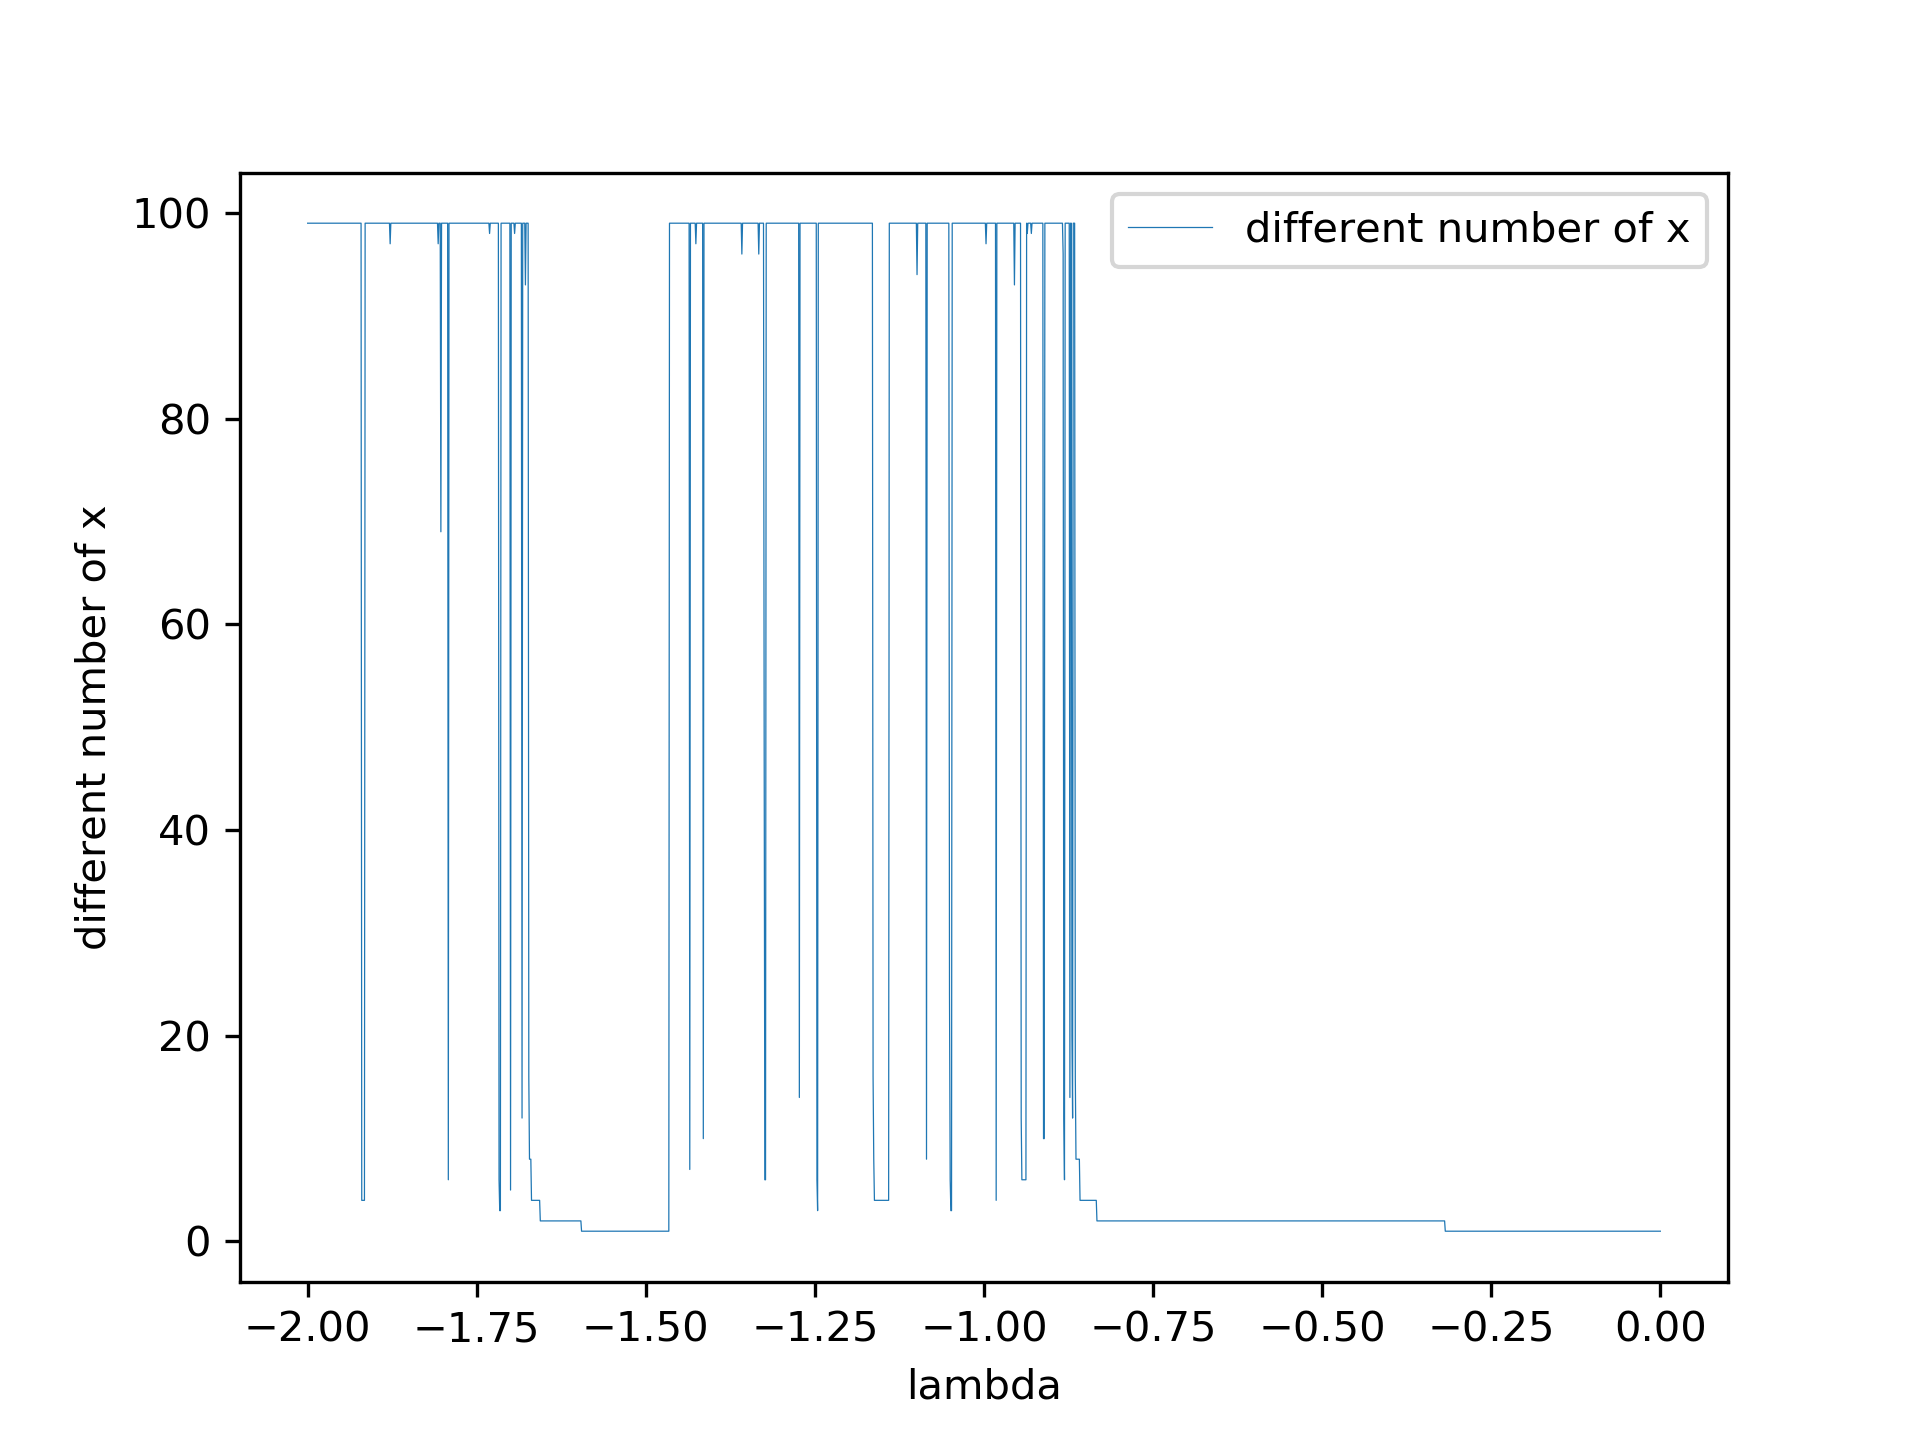
\includegraphics[bb= 0 0 450 370,width=9cm]{s=0.001-2-1.png}      
\caption{ 输出迭代后100个结果,$step = 0.001$,$\lambda \in [-2,0]$的迭代不同结果个数-$\lambda$曲线}      
\end{figure}



\begin{figure}[!htbp]        
\centering
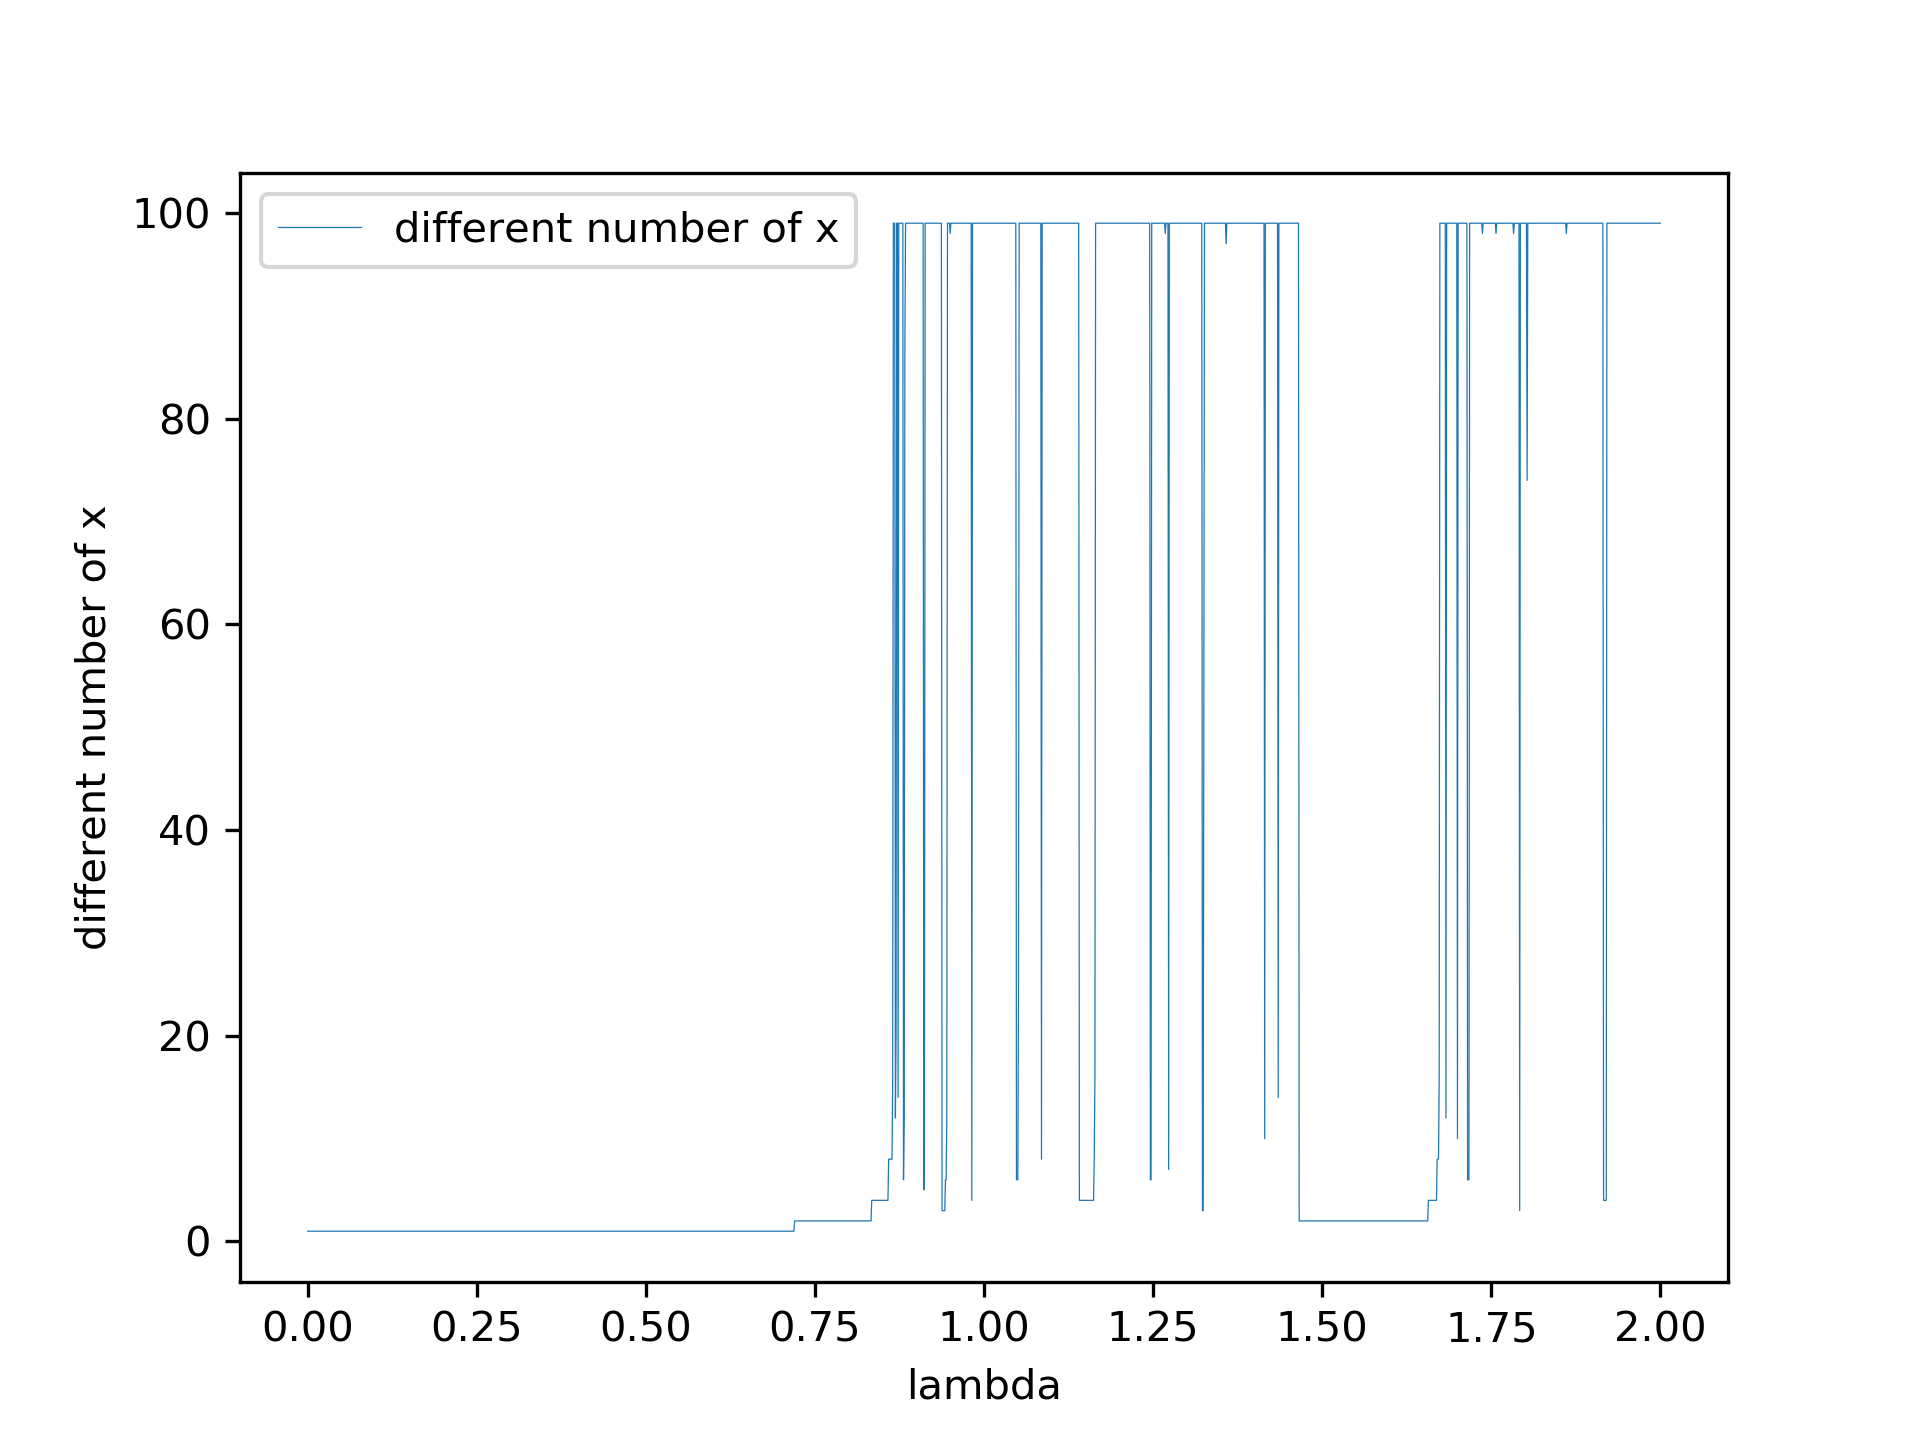
\includegraphics[bb= 0 0 450 370,width=9cm]{s=0.001-3-1.png}      
\caption{输出迭代后100个结果,$step = 0.001$,$\lambda \in [0,2]$的迭代不同结果个数-$\lambda$曲线}      
\end{figure}



\subsection{Feigenbaum 常数的计算}
为了计算Feigenbaum 常数,我们利用Python脚本\footnote{具体代码见附录}对不同$\lambda$取值输出的后100个迭代值进行分析。对于常数$\delta$,对结果的不同值进行个数统计,找到不同个数的不动点所对应的参数$\lambda$取值。然后不断缩小区间,加大精度来找到比较精确的分岔值$\lambda_{m}$。这里省略具体的过程,只给出最后的结果:


\begin{table}[!htbp]
\centering
\resizebox{\textwidth}{!}{
\begin{tabular}{|c|c|c|c|}
\hline
m  &分叉情况     &分岔值$\lambda_{m}$  &Feigenbaum 常数$\delta$ \\ \hline
1  &1 $\rightarrow$ 2    &-0.3183122   & \\ \hline
2  &2 $\rightarrow$ 4    &-0.8332658  &20.31936 \\ \hline
3  &4 $\rightarrow$ 8   &-0.858608  &4.62852 \\ \hline
4  &8 $\rightarrow$ 16  &-0.8640842  &4.66095 \\ \hline
5  &16 $\rightarrow$ 32  &-0.86525894  &4.66611 \\ \hline
6  &32 $\rightarrow$ 64  &-0.8655107  & \\ \hline
\end{tabular}}
\caption{$\lambda < 0$时的Feigenbaum常数$\delta$计算结果}
\end{table}


\begin{table}[!htbp]
\centering
\resizebox{\textwidth}{!}{
\begin{tabular}{|c|c|c|c|}
\hline
m  &分叉情况     &分岔值$\lambda_{m}$  &Feigenbaum 常数$\delta$ \\ \hline
1  &1 $\rightarrow$ 2    &0.7199599   & \\ \hline
2  &2 $\rightarrow$ 4    &0.8332658  &4.47090 \\ \hline
3  &4 $\rightarrow$ 8   &0.8586088  &4.62852 \\ \hline
4  &8 $\rightarrow$ 16  &0.8640842  &4.66071 \\ \hline
5  &16 $\rightarrow$ 32  &0.865259  &4.66746 \\ \hline
6  &32 $\rightarrow$ 64  &0.8655107  & \\ \hline
\end{tabular}}
\caption{$\lambda > 0$时的Feigenbaum常数$\delta$计算结果}
\end{table}

\newpage
与Feigenbaum常数理论值$\delta = 4.669201609 \cdots$比较,看出除$\lambda < 0 $情况下的$\frac{\lambda_{2}-\lambda_{1}}{\lambda_{3}-\lambda_{2}}$以外,计算模拟值与理论值误差比较小。具体为何$\lambda < 0 $情况下的$\frac{\lambda_{2}-\lambda_{1}}{\lambda_{3}-\lambda_{2}}$与理论值相差较大,目前本人并不清楚。另外注意到,参数$\lambda$大于0和小于0的时候,分岔值除了$\lambda_{1}$其他的基本一致,而小于0的情形下,与$\lambda_{1}$有关的Feigenbaum常数$\delta$计算值与理论值偏差很大。

由于$\lambda<0$时的情况有些复杂\footnote{本人发现对于一些分岔值并不会与0.5相交,几乎相交线只与混沌区中的某些值相交},但是与$>0$方法差不多,故下面只讨论$\lambda>0$的情况
对于Feigenbaum常数$\alpha$的值,我们也如法炮制,不断缩小区间,加大精度,看输出结果与0.5的差值小于某个值时,认为此时与0.5相交,认为此值为$\lambda_{m}$

\begin{comment}
	
\begin{table}[!htbp]
\centering
\resizebox{\textwidth}{!}{
\begin{tabular}{|c|c|c|c|c|}
\hline
m  &分叉情况     &分岔值$\lambda_{m}$ & $d_{m}$    &Feigenbaum 常数$\alpha$ \\ \hline
1  &1 $\rightarrow$ 2    &-0.500000   & \\ \hline
2  &2 $\rightarrow$ 4    &-0.776244 &1.27807469 \\ \hline
3  &4 $\rightarrow$ 8   &  & \\ \hline
4  &8 $\rightarrow$ 16  &  & \\ \hline
5  &16 $\rightarrow$ 32  &  & \\ \hline
6  &32 $\rightarrow$ 64  &  & \\ \hline
\end{tabular}}
\caption{$\lambda > 0$时的Feigenbaum常数计算结果}
\end{table}

\end{comment}


\begin{table}[!htbp]
\centering
\resizebox{\textwidth}{!}{
\begin{tabular}{|c|c|c|c|c|}
\hline
m      &与0.5相交值$\lambda_{m}$  & $d_{m}$    &Feigenbaum 常数$\alpha$ \\ \hline
0   &0.500000    &   		 & \\ \hline
1   &0.7777338   &0.27773377 &  \\ \hline
2   &0.84638217  &0.10720426 &2.590697142072526  \\ \hline
3   &0.86145035  &0.04251802 &2.521384109608114 \\ \hline
4   &0.864694181 &0.01696186 &2.506683818873638 \\ \hline
\end{tabular}}
\caption{$\lambda > 0$时的Feigenbaum常数$\alpha$计算结果}
\end{table}

与理论值$\alpha = 2.502 907 875\cdots$比较可看出随着$\lambda_{m}$的精度提高,其计算值与理论值偏差越小,基本验证此常数值。



\subsection{关于分岔值计算时的方法讨论}
一般情况下,我们理所当然的认为将输出结果输入到分析脚本中,判断结果和之前的结果均不同时,结果种类数$+1$。但实际操作中,发现这样处理数据会出现一些问题。例如我们改变输出结果的精度时,统计结果会出现偏差:

\begin{figure}[!htbp]        
\centering
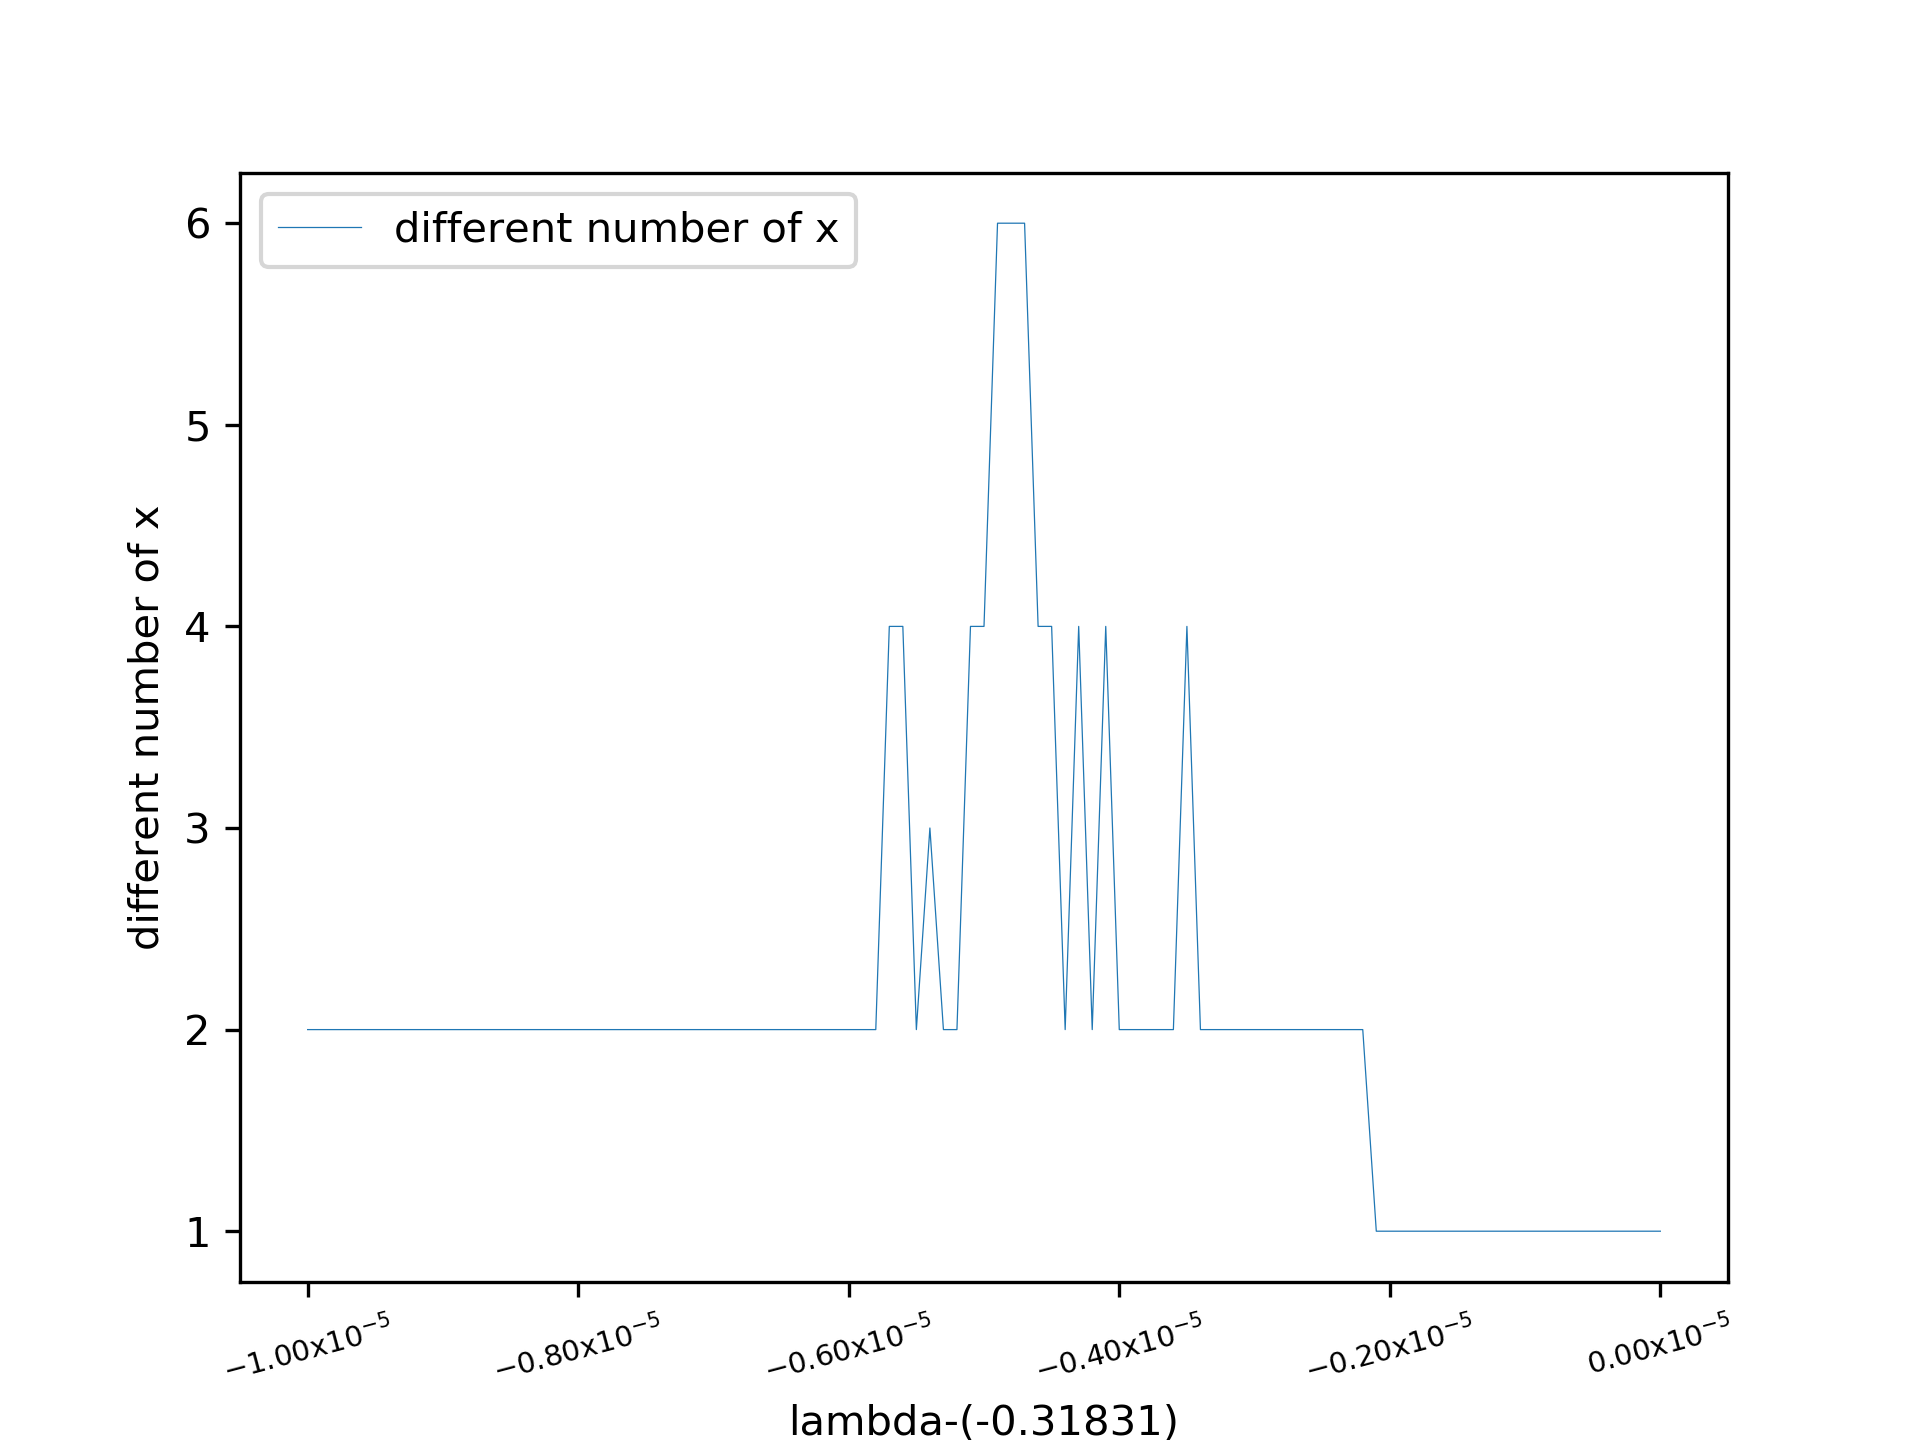
\includegraphics[bb= 0 0 450 370,width=9cm]{7-6.png}      
\caption{输出结果保留6位小数时,$step = 10^{-7}$,$\lambda \in [-0.31832,-0.31831]$的迭代不同结果个数-$\lambda$曲线}      
\end{figure}


\begin{figure}[!htbp]        
\centering
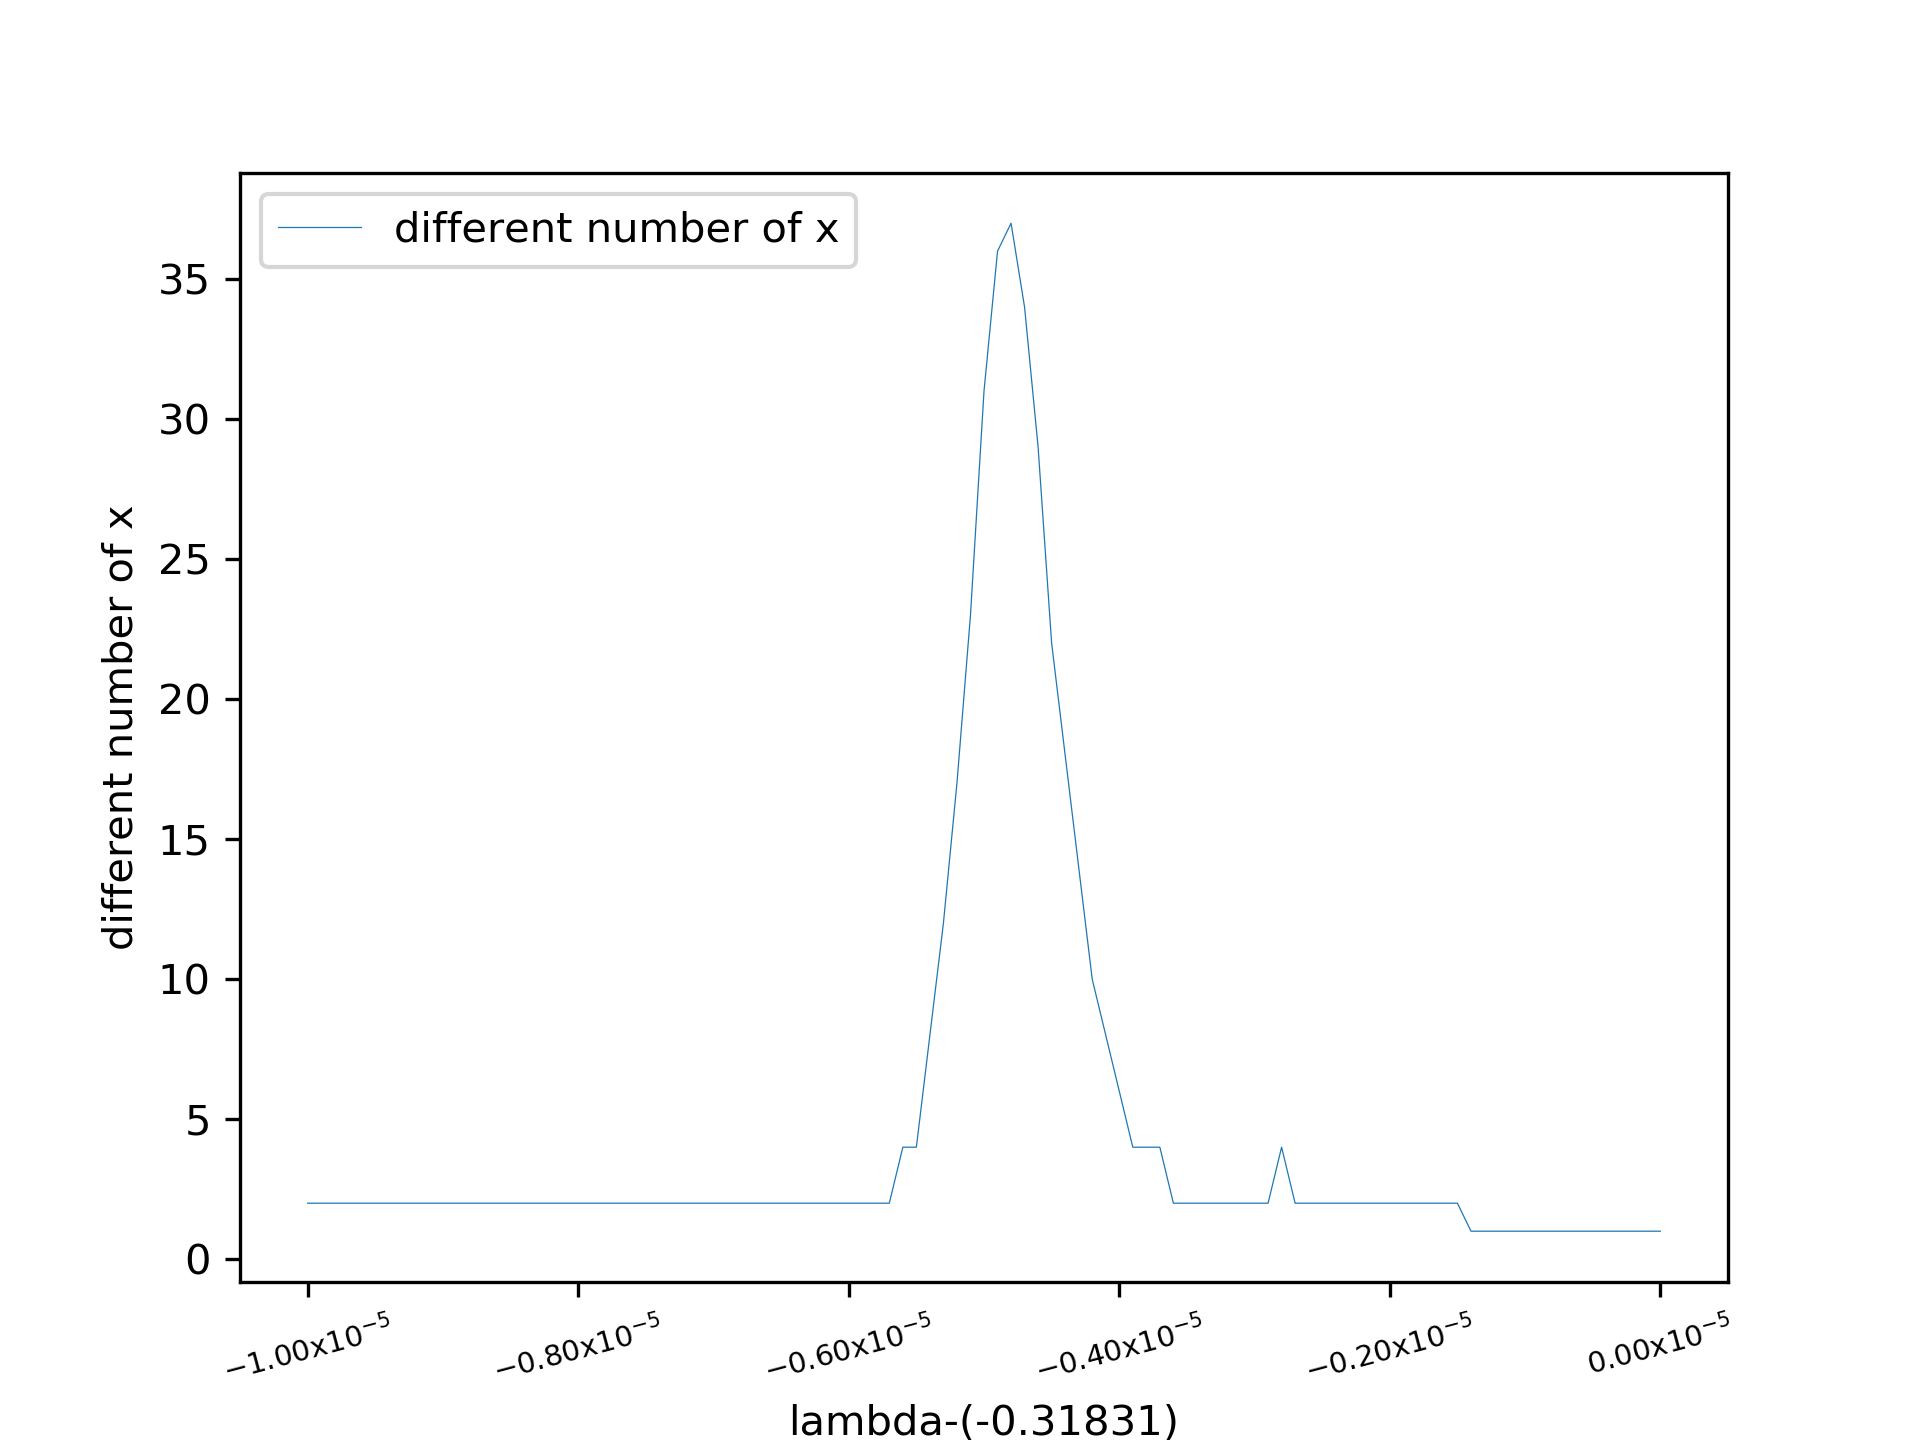
\includegraphics[bb= 0 0 450 370,width=9cm]{7-7.png}      
\caption{输出结果保留7位小数时,$step = 10^{-7}$,$\lambda \in [-0.31832,-0.31831]$的迭代不同结果个数-$\lambda$曲线}      
\end{figure}

\newpage
但实际上,对此区间的迭代结果进行可视化绘图得到

\begin{figure}[!htbp]        
\centering
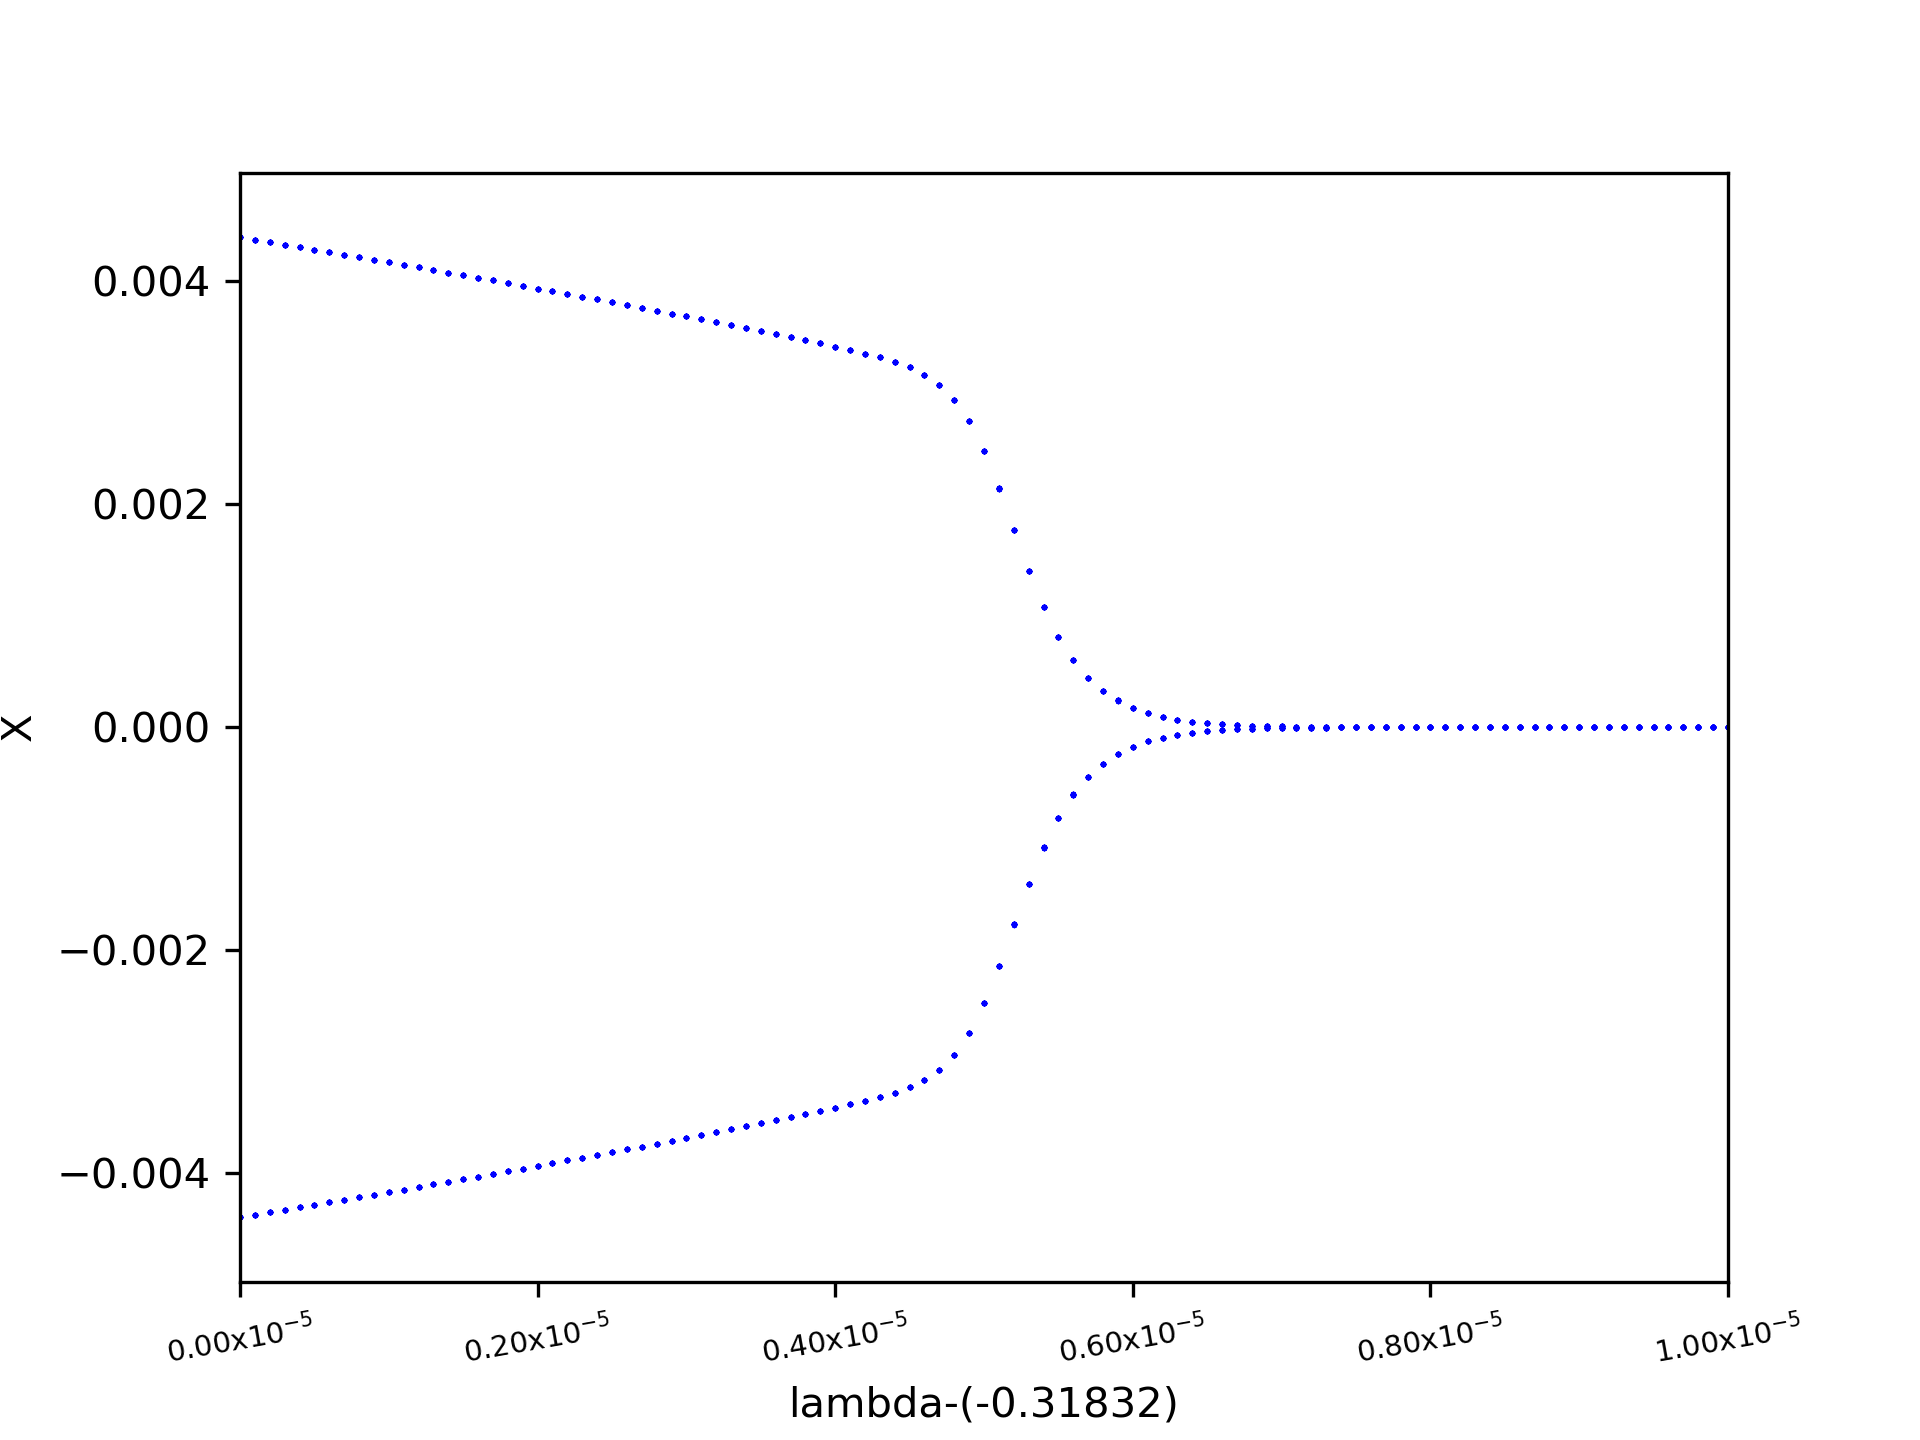
\includegraphics[bb= 0 0 450 370,width=9cm]{7-7-1.png}      
\caption{输出结果保留7位小数时,$step = 10^{-7}$,$\lambda \in [-0.31832,-0.31831]$的迭代结果可视化}      
\end{figure}


明显看出此区间内为绝灭到2分岔值的转变,并无更高分岔值的转变。利用脚本分析分岔值出现这种问题的原因可能为程序迭代时不可避免的出现了一些很小的舍入误差,故造成本该相同的值输出值不同。所以对于分岔很多的情况下,必须考虑减小计算机迭代过程中出现的各种误差,从而得到正确的分岔值。

\section{心得与体会}
通过此次作业,对混沌和Feigenbaum常数有了更深的认识。另外注意到在程序中比如类似(以C语言的for循环示意)for(y = min;y < max+step;y += step)的循环,当step很小的时候,由于计算机的误差,可能会导致此循环进行y = max+step 的步骤。所以循环应改为for(y = min;y < max+step/2;y += step),这样才能保证程序进行我们希望计算的循环。寻找分岔值时,也体会到数值计算误差带来的一些事情需要特别小心注意。 


\newpage
\section{附录}

\begin{appendices}

\section{C语言源程序}
\begin{lstlisting}[language = C]
#include <stdio.h>
#include <stdlib.h>
#include <math.h>
#include <string.h>
#define Pi 3.1415926535

int my_filewriter_double(char str1[],char str2[],double num[],double y,int n){
    FILE * fp;
    char str[20];
    strcpy(str,str1);
    strcat(str,str2);
    fp = fopen(str,"a+");

    for(int i=0;i<(n);i++)
    {
        fprintf(fp,"%lf,%lf\n",y,num[i]);

    }
    fclose(fp);
    return 0;
}



int my_fiter(double x[],int N,int n,double y,double x0){
    double temp = x0;  //迭代初值
    for(int i =0;i<N-n;i++){
        temp = y*sin(Pi*temp);
    }
    
    for(int i =0;i<n;i++){  //要输出的结果进行幅值
        temp = y*sin(Pi*temp);
        x[i] = temp;
    }
    
    return 0;
}



int main(int argc, const char * argv[]) {
    double min = 0.86551;  //lambda的最小值
    double max = 0.86552;   //lambda的最大值
    int N = 1000000;   //迭代次数
    int n = 100;   //输出迭代结果的后多少个结果
    double step = 0.0000001;  //不同lambda之间的间隔
    
    double *x = malloc(sizeof(double)*n);
    
    for(double y = min;y < max + (step/(double)2);y += step){ //y为迭代参数lambda
        my_fiter(x, N, n, y, 15);  //迭代初值选为15
        my_filewriter_double("", "x.dat", x, y, n);
    }
    
    return 0;
}

\end{lstlisting}

\newpage

\section{可视化绘图及数据分析Python程序源码}

\begin{lstlisting}[language = python]
import matplotlib.pyplot as plt
import numpy as np
import math
import csv
#from IPython.core.pylabtools import figsize # import figsize
plt.rcParams['savefig.dpi'] = 300 #图片像素
plt.rcParams['figure.dpi'] = 300 #分辨率
# 默认的像素:[6.0,4.0],分辨率为100,图片尺寸为 600&400
fig1 = plt.figure()
fig2 = plt.figure()

ax1 = fig1.add_subplot(111)
ax2 = fig2.add_subplot(111)

step = 0.0000001  # 每个lambda取值之间的间隔
max = 0.86552   # lambda的取值区间
min = 0.86551

X = []
Y = []
X1 = []
Y1 = []
flag = 0
i = 0
temp1 = []
temp = 0

csv_file = csv.reader(open('problem 12/x.dat', 'r'))
for line in csv_file:
    [tempX, tempY] = line
    i += 1
    if i % 100 == 0 and i != 0:  # 每读100行数据,进行统计(因为C程序输出后100个迭代值)
        temp2 = set(temp1)  # 因为此步骤考虑不同lambda值对应的输出x值中的不同结果数,
 # 故变为集合形式,使其中只有不同的元素,然后其长度即代表所求
        temp = len(temp2)
        Y1.append(len(temp2))  # 记录不同lambda值对应的输出x值中的不同结果数
        temp1 = []
    else:
        temp1.append(float(tempY))

    X.append(float(tempX))  # lambda 的值
    Y.append(float(tempY))  # 与相应lambda对应的输出结果


X = np.array(X)
Y = np.array(Y)


ax1.scatter(X, Y, c='b', label='', s=0.1, alpha=0.5, marker='o')  # x-lambda散点图
ax1.set_xlabel('lambda')
ax1.set_ylabel('X')
fig1.savefig("1.png")

X1 = np.arange(min, max + step/2, step)

ax2.plot(X1, Y1, lw=0.3, label='different number of x')  # x不同结果数-lambda折线图
ax2.legend(loc=2)
ax2.set_xlabel('lambda')
ax2.set_ylabel('different number of x')
fig2.savefig("2.png")

if max < 0:
    Y1.reverse()  # 当参数lambda<0时,需对Y1 List 进行排序上的反转,>0时此步骤不运行


flag = 0

for i in Y1:   # 输出 lambda值及其对应的输出结果中的x的种类数(用来找分岔值)
    if flag < 1001:
        print(min + flag*step, "\t", i)  # 前面为lambda值,后面为其对应的输出结果中的x的结果数
    flag += 1



\end{lstlisting}


\end{appendices}




\end{document}
